Una volta discusse le caratteristiche generali dei rivelatori possiamo entrare più nel dettaglio, andando a studiare le diverse tipologie di rivelatori.

Cominciamo dai rivelatori a gas, in quanto storicamente questi sono stati i primi rivelatori ad essere stati sviluppati. Ancora oggi questi vengono adoperati non solo nel campo della ricerca, ma anche in alcuni campi applicativi come il campo medico.

\section{Principio di funzionamento}

Il principio di funzionamento dei rivelatori a gas si basa sul fenomeno della ionizzazione, in quanto essi sono dei rivelatori che contengono al loro interno un gas.

\begin{figure}[H]
   \centering
   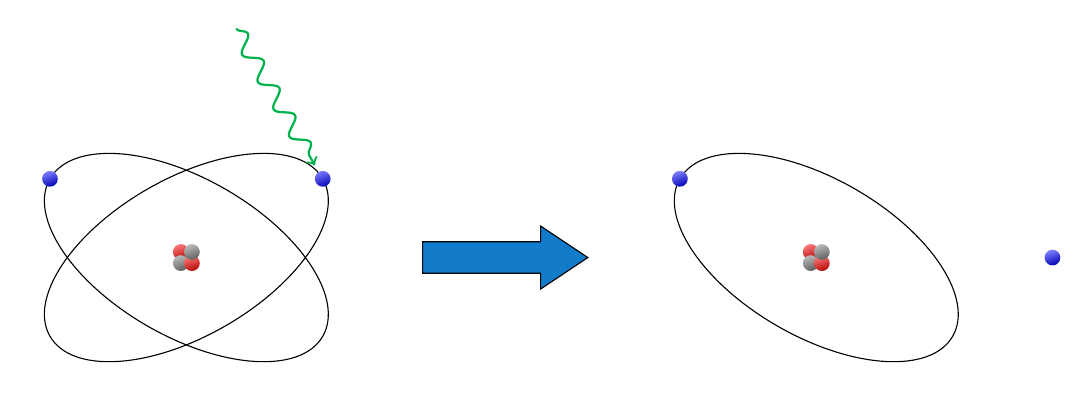
\begin{tikzpicture}
      %nucleo
      \shade[rotate=45,top color=red!50,bottom color=red!70!black,shading angle=20] (0,0.1) circle (0.1cm);
      \shade[rotate=45,top color=gray!50,bottom color=gray!70!black,shading angle=20] (-0.1,0) circle (0.1cm);
      \shade[rotate=45,top color=red!50,bottom color=red!70!black,shading angle=20] (0,-0.1) circle (0.1cm);
      \shade[rotate=45,top color=gray!50,bottom color=gray!70!black,shading angle=20] (0.1,0) circle (0.1cm);
      %orbite
      \draw[rotate=30] (0,0) ellipse (2cm and 1cm);
      \shade[rotate=30,top color=blue!50,bottom color=blue!70!black,shading angle=20] (2,0) circle (0.1cm);
      \draw[rotate=150] (0,0) ellipse (2cm and 1cm);
      \shade[rotate=150,top color=blue!50,bottom color=blue!70!black,shading angle=20] (2,0) circle (0.1cm);
      %fotone
      \draw[->,thick, teal!60!green, decorate, decoration={snake, segment length=4mm, amplitude=1mm,post length=1mm},rotate=30,rotate around={90:(2,0)}] (4.2,0) -- (2.2,0);
      %freccia
      \draw [fill=cyan!60!blue!,shift={(2.5 cm,0 cm)}] (0.5,0.2) -- (2,0.2) -- (2,0.4) -- (2.6,0) -- (2,-0.4) -- (2, - 0.2) -- (0.5,-0.2) -- cycle;
      \begin{scope}[shift={(8cm, 0cm)}]
        %nucleo
        \shade[rotate=45,top color=red!50,bottom color=red!70!black,shading angle=20] (0,0.1) circle (0.1cm);
        \shade[rotate=45,top color=gray!50,bottom color=gray!70!black,shading angle=20] (-0.1,0) circle (0.1cm);
        \shade[rotate=45,top color=red!50,bottom color=red!70!black,shading angle=20] (0,-0.1) circle (0.1cm);
        \shade[rotate=45,top color=gray!50,bottom color=gray!70!black,shading angle=20] (0.1,0) circle (0.1cm);
        %orbite
        \draw[rotate=150] (0,0) ellipse (2cm and 1cm);
        \shade[rotate=150,top color=blue!50,bottom color=blue!70!black,shading angle=20] (2,0) circle (0.1cm);
        %elettrone
        \shade[top color=blue!50,bottom color=blue!70!black,shading angle=20] (3,0) circle (0.1cm);
      \end{scope}
    \end{tikzpicture}
\end{figure}

%L'idea alla base è quella di sfruttare il fatto che le particelle che attraversano un contenitore pieno di gas cedono energia e la possono cedere andando a produrre fenomeni di ionizzazione. Quindi sostanzialmente l'energia ricevuta da uno degli elettroni degli atomi che compongono il gas permette all'elettrone di essere espulso e quindi alla fine il risultato è la produzione di una coppia ione positivo-elettrone.
Il concetto di base è sfruttare il fatto che le particelle che attraversano un contenitore pieno di gas trasferiscono energia, che può essere utilizzata per produrre fenomeni di ionizzazione. In pratica, l'energia assorbita da uno degli elettroni degli atomi del gas permette ad esso di essere espulso, generando così una coppia composta da uno ione positivo e un elettrone libero.

\begin{minipage}{0.35\textwidth}
   \begin{figure}[H]
      \centering
      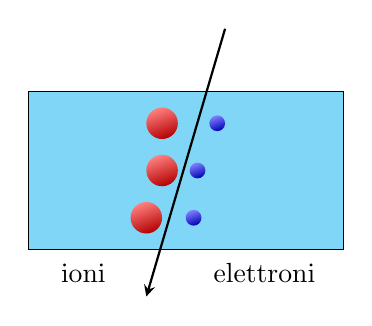
\begin{tikzpicture}
         %gas
         \draw[fill=cyan!50!white!] (0,-1) -- (0,1) -- (4,1) -- (4,-1) -- cycle;
         \draw[-stealth,thick] (2.5,1.8) -- (1.5,-1.6);
         %particelle
         %prima fila
         \shade[top color=red!50,bottom color=red!70!black,shading angle=20] (1.7,0.6) circle (0.2cm);
         \shade[top color=blue!50,bottom color=blue!70!black,shading angle=20] (2.4,0.6) circle (0.1cm);
         %seconda fila
         \shade[top color=red!50,bottom color=red!70!black,shading angle=20] (1.7,0) circle (0.2cm);
         \shade[top color=blue!50,bottom color=blue!70!black,shading angle=20] (2.15,0) circle (0.1cm);
         %terza fila
         \shade[top color=red!50,bottom color=red!70!black,shading angle=20] (1.5,-0.6) circle (0.2cm);
         \shade[top color=blue!50,bottom color=blue!70!black,shading angle=20] (2.1,-0.6) circle (0.1cm);
         %nomi
         \node at (0.7,-1.3) {ioni};
         \node at (3,-1.3) {elettroni};
       \end{tikzpicture}
   \end{figure}
\end{minipage}
\begin{minipage}{0.64\textwidth}
   \vspace{0.7cm}Possiamo schematizzare un rivelatore al gas come un contenitore riempito di gas. Nel momento in cui passa una particella carica, questa particella produce coppie elettrone-ione, i quali hanno dimensioni e masse notevolmente differenti, fatto che comporta delle conseguenze soprattutto per quello che riguarda la raccolta del segnale. 
\end{minipage}

Chiaramente, nel momento in cui una particella attraversa un volume pieno di gas non viene prodotta una sola coppia: ne vengono prodotte un certo numero che dipende da quanta energia la particella deposita all'interno del gas.

Un tale sistema funziona come rivelatore perché abbiamo un segnale (che in questo caso è la produzione di coppie elettrone-ione) che indica il passaggio di una particella. Addirittura, se fossimo capaci di contare quante coppie sono state create potremmo avere un'informazione anche sull'energia che è stata depositata all'interno del rivelatore. 

Questi rivelatori a gas possono essere adoperati sia in current mode che in pulsed mode. La differenza sta nel fatto che in pulsed mode si produce un impulso elettrico ogni volta che passa una particella, mentre nella modalità current mode il flusso di particelle è così elevato che alla fine si produce una corrente continua il cui valore è proporzionale al flusso di particelle che sta incidendo sul rivelatore, dunque è come se si facesse una media di tanti impulsi che sono molto ravvicinati tra di loro in tempo, quindi non è più possibile distinguere un impulso dal successivo, ma si ha sostanzialmente una corrente continua.

\section{Ionizzazione}

\subsection{Meccanismi di interazione}

I processi di interazione di una particella carica in un gas si dividono essenzialmente in due tipi di reazione:
\begin{enumerate}
   \item eccitazione;
   \item ionizzazione, in cui vengono creati un elettrone libero e uno ione.
\end{enumerate}
L'eccitazione di un atomo $X$ ad opera di una particella carica $p$ è
\begin{equation*}
   X + p \ce{->} X^* + p
\end{equation*}
ed è una reazione risonante, che richiede il trasferimento di un corretto valore di energia, in quato il valore di energia fornito deve corrispondere al salto energetico dell'elettrone.

Le sezioni d'urto tipiche nei gas nobili in risonanza sono dell'ordine di $\sigma \approx 10^{-17} \; \text{cm}^2$. Sebbene non vengano creati elettroni o ioni liberi, le molecole o gli atomi eccitati possono partecipare a ulteriori reazioni che portano alla ionizzazione.

%\comment{
\begin{approfondimento}[Le reazioni risonanti]
   \footnotesize
   Una "reazione risonante" è un concetto utilizzato in fisica, in particolare nel contesto delle reazioni nucleari e delle reazioni chimiche, per descrivere un fenomeno in cui la probabilità di una reazione aumenta notevolmente a causa della presenza di una "risonanza".
   
   Nel contesto delle reazioni nucleari, una reazione risonante si verifica quando l'energia dei nuclei che partecipano alla reazione corrisponde all'energia di uno stato eccitato (risonanza) del nucleo composto che si forma temporaneamente durante la reazione. Questo stato eccitato è di solito instabile e si disintegra rapidamente, ma la coincidenza tra l'energia dei reagenti e l'energia dello stato eccitato aumenta significativamente la probabilità che la reazione avvenga. In pratica, la sezione d'urto (una misura della probabilità di reazione) ha un picco molto alto a una specifica energia, corrispondente all'energia della risonanza. Questo fenomeno è comune nelle reazioni nucleari a basse energie, come quelle che avvengono nelle stelle o nei reattori nucleari.

   L'eccitazione è considerata una reazione risonante in alcuni contesti perché coinvolge un trasferimento di energia che coincide con l'energia specifica necessaria per portare un sistema (come un atomo o un nucleo) in uno stato eccitato, che è uno stato di energia superiore rispetto al suo stato fondamentale.

   I motivi per cui si parla di "risonanza" nel contesto dell'eccitazione sono i seguenti:
   \begin{enumerate}[leftmargin=0.5cm]
      \item Coincidenza Energetica: L'eccitazione avviene quando l'energia di una particella incidente (come un fotone o un elettrone) corrisponde esattamente all'energia di uno stato eccitato del sistema. Questa coincidenza energetica è una condizione di risonanza. Ad esempio, se un atomo assorbe un fotone la cui energia corrisponde alla differenza tra due livelli energetici dell'atomo, l'atomo può essere eccitato a uno stato superiore.
      \item Massima Probabilità di Assorbimento: Quando l'energia della particella incidente coincide con l'energia del livello eccitato, la probabilità che il sistema assorba l'energia e si ecciti è massima. Questo è analogo a ciò che accade nelle reazioni nucleari risonanti, dove la sezione d'urto raggiunge un picco a una certa energia.
      \item Effetto di Risonanza: La "risonanza" si riferisce alla condizione in cui un sistema risponde con un'amplificazione del segnale o dell'energia in ingresso quando quest'ultima corrisponde a una delle frequenze naturali del sistema. Nel caso dell'eccitazione, il sistema atomico o molecolare risponde fortemente (cioè si eccita) quando l'energia fornita è in risonanza con una delle sue frequenze naturali (o stati energetici quantizzati).
   \end{enumerate}
   In sintesi, l'eccitazione è una reazione risonante perché avviene più facilmente quando l'energia fornita corrisponde esattamente all'energia richiesta per raggiungere uno specifico stato eccitato del sistema, massimizzando così la probabilità di assorbimento e la conseguente eccitazione.
\end{approfondimento}
%}

Per una ionizzazione, che è
\begin{equation*}
   X + p \ce{->} X^+ + e^- + p
\end{equation*}
non esiste, naturalmente, un requisito energetico esatto e, in effetti, la sua sezione d'urto è leggermente superiore con $\sigma \approx 10^{-16} \; \text{cm}^2$. Tuttavia, il processo di ionizzazione avviene solamente se l'energia fornita supera una certa soglia, perché è necessario che l'elettrone venga strappato, quindi bisogna almeno fornire un'energia pari all'energia di prima ionizzazione del gas che stiamo adoperando.

Possiamo quindi dire che nella maggior parte dei casi avviene ionizzazione e ciò è probabilmente legato al fatto che l'energia per eccitare un elettrone non può assumere qualsiasi valore ma deve assumere dei valori ben precisi\footnote{Il Leo la pensa in maniera diametralmente opposta: dice che "La ionizzazione ha una soglia di energia relativamente alta e, poiché i trasferimenti di energia a basso valore sono più probabili, le reazioni di eccitazione generalmente prevalgono.", quindi non so a chi credere.}.

Gli elettroni e gli ioni creati dalla radiazione incidente stessa sono noti come ionizzazione primaria. In alcuni di questi casi di ionizzazione, tuttavia, viene trasferita una quantità di energia sufficientemente grande all'elettrone (raggi delta), tale che questo elettrone crea a sua volta coppie ione-elettrone. Quest'ultima ionizzazione è nota come ionizzazione secondaria. Se la loro energia è sufficientemente alta, gli elettroni di ionizzazione secondaria possono ionizzare ulteriormente, e così via fino a raggiungere la soglia per le reazioni di ionizzazione.

\comment{Se guardiamo i meccanismi di interazione delle particelle in un gas, scopriamo in realtà non sono possibili soltanto processi di ionizzazione degli atomi e delle molecole che compongono il gas, ma è possibile anche che si verifichi un fenomeno di eccitazione. Quindi andando a guardare alle tipologie di interazioni che possono avvenire, possiamo avere o che la particella X cede una porzione della sua energia che è in grado di eccitare l'elettrone e quindi portarlo a un livello eccitato (e oppure è possibile, come abbiamo detto prima, andare a ionizzare la molecola o l'atomo del gas e quindi produrre una coppia $\text{X}^+ - e^+$. Questo . In termini di sezione d'urto possiamo dire che i processi di ionizzazione sono processi più frequenti, più probabili, perché abbiamo una sezione d'urto dell'ordine di $10^{-16} \; \rm cm^2$, in confronto ai processi di eccitazione che hanno una sezione d'urto dell'ordine di $10^{-17} \; \rm cm^2$. Quindi, a seguito del processo di ionizzazione si producono delle particelle, in particolare elettroni e ioni, che a loro volta in determinate condizioni potrebbero innurre e nascare dei fenomeni di ionizzazioni secondarie. Quindi abbiamo sia dei prodotti diretti di prima ionizzazione sia eventualmente dei prodotti secondari. Ora vedremo in che condizioni si innescano questi processi secondari.}

\subsection{W-values}
Ci chiediamo adesso quante coppie di ioni ed elettroni si formano. Siamo particolarmente interessati a questa informazione perché il numero di coppie ci potrebbe dare un'informazione sull'energia depositata.

Ingenuamente potremmo pensare che il numero medio di coppie che si formano siano date dal rapporto tra l'energia depositata e il potenziale di prima ionizzazione di un gas, il quale assume valori compresi tra i 10 e i 25 eV a seconda del tipo di gas che stiamo adoperando. Ciò sarebbe corretto se avvenissero soltanto ionizzazioni, ma nella realtà avviene anche l'eccitazione, per cui nel valutare il numero di coppie ione-elettrone che si formano dobbiamo tenere conto del fatto che parte dell'energia che viene depositata viene utilizzata per eccitare gli elettroni, quindi non viene totalmente adoperata per la ionizzazione, cioè per creare coppie. Ecco perché l'energia media per creare una coppia ione-elettrone è un po' più alta rispetto al potenziale di prima ionizzazione, variando normalmente tra i 25 e i 40 eV.

\begin{figure}[H]
   \centering
   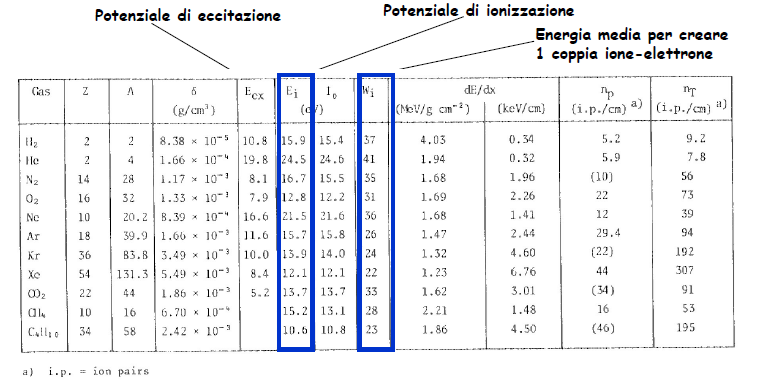
\includegraphics[width=\textwidth]{immagini/potenziali_ionizzazione.png}
\end{figure}

In questa tabella possiamo vedere, per diverse tipologie di gas, i valori del potenziale di eccitazione e di prima ionizzazione, indicati rispettivamente con $E_{\rm ex}$ e $E_{\rm i}$, e l'energia media per creare una coppia ione-elettrone, indicata con $W$. Notiamo che per eccitare gli atomi sono necessarie energie dell'ordine della decina di elettronVolt, mentre, per ionizzare, il potenziale di prima ionizzazione assume valori un po' più alti, tra i 10 e i 20 eV. Se invece consideriamo l'energia media per creare una coppia ione-elettrone, questa risulta essere un po' più grande rispetto al potenziale di prima ionizzazione, in quanto tiene conto dei fenomeni di eccitazione. Se ad esempio utilizzassimo dell'idrogeno $\rm H_2$, l'energia media per creare una coppia è pari a 37 eV.

\vspace{0.4cm}

\begin{minipage}{0.245\textwidth}
   \begin{center}
      \begin{tabular}{|c|c|}
         \hline
         &\\[-0.4cm]
         Gas & $W$ (eV)\\[0.1mm]
         &\\[-0.4cm]
         \hline
         &\\[-0.4cm]
         Ne & $36.3$\\[0.1mm]
         \hline
         &\\[-0.4cm]
         Ar & $26.2$\\[0.1mm]
         \hline
         &\\[-0.4cm]
         Xe & $21.5$\\[0.1mm]
         \hline
         &\\[-0.4cm]
         $\rm P10$ & $26$\\[0.1mm]
         \hline
      \end{tabular}
   \end{center}
\end{minipage}
\begin{minipage}{0.75\textwidth}
   \vspace{0.1cm}L'energia media per creare una coppia $W$ è quella che ci permette di stimare quante coppie elettrone-ione si formano all'interno di un gas. Il valore di $W$ dipende dal tipo di gas, ad esempio nella tabella a fianco possiamo vedere i valori per dei gas nobili, in quanto spesso nei rivelatori a gas si utilizzano gas nobili, ma si utilizzano tante volte anche delle miscele come il $\rm P10$, che è una composizione di argon al 90\% e di metano ($\rm CH_4$) al 10\%.
\end{minipage}

\vspace{0.4cm}

In realtà il valore di $W$ dipende leggermente anche dal tipo di particella e dall'energia. Nel seguente grafico vediamo un esempio di valori di $W$ per diverse particelle incidenti in funzione dell'energia:

\begin{figure}[H]
   \centering
   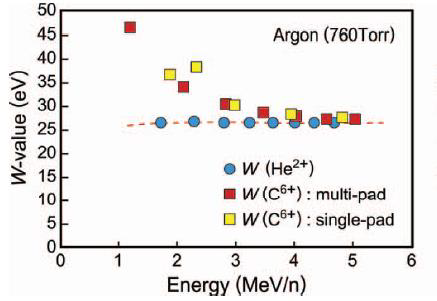
\includegraphics[width=0.6\textwidth]{immagini/vallori_W_energia.png}
\end{figure}

Vediamo che c'è una leggerissima dipendenza dall'energia e dal tipo di particella, quindi non è sufficiente conoscere solamente il gas, ma in realtà purtroppo questo valore può dipendere leggermente anche dalla particella.

Inoltre, nel caso in cui si adopera una miscela di gas, per valutare il valore del potenziale medio per creare la coppia si utilizza una sorta di media pesata, un po' come abbiamo visto nel caso della perdita di energia nei composti.

\begin{approfondimento}[W-values per miscele e numero di coppie]
   \footnotesize
   Metto questo approfondimento perché la professoressa non spiega esplicitamente come calcolarlo. Come al solito ringraziamo chatgpt.\\[0.2cm]
   Se abbiamo una miscela di gas, il $W$-value della miscela può essere calcolato in base ai $W$-value dei singoli componenti della miscela e alle loro frazioni molari o volumetriche. L'espressione generale è data da
   \begin{equation*}
      W_{\text{mix}} = \frac{1}{\sum_i \frac{x_i}{W_i}}
   \end{equation*}
   dove $W_{\text{mix}}$ è il $W$-value della miscela di gas e $x_i$ e $W_i$ sono rispettivamente la frazione molare o volumetrica e il $W$-value del componente $i$-esimo nella miscela.\\
   \comment{Se ad esempio abbiamo una miscela composta da due gas, A e B, con frazioni volumetriche $x_A$ e $x_B$ rispettivamente, e $W$-value $W_A$ e $W_B$, il $W$-value della miscela sarebbe:
   \begin{equation*}
      W_{\text{mix}} = \frac{1}{\frac{x_{\rm A}}{W_{\rm A}} + \frac{x_{\rm B}}{W_{\rm B}}}
   \end{equation*}
   Questo calcolo può essere esteso a miscele con più di due componenti, semplicemente aggiungendo più termini nella somma.\\}
   \E da notare che il $W$-value dipende dalle proprietà fisiche del gas e dalle condizioni operative, come la pressione e la temperatura. Tuttavia, in prima approssimazione, la formula sopra riportata è utile per calcolare il valore $W$ di una miscela a condizioni standard.\\[0.2cm]
   \textbf{$\boldsymbol{W}$-value per unità di percorso}\\
   Il $W$-value si può esprimere anche in termini di unità di percorso (ad esempio, per calcolare l'energia media necessaria per creare una coppia di ioni per unità di lunghezza percorsa da una particella carica in un gas). Per fare ciò, si può utilizzare una relazione che coinvolge la perdita di energia per unità di lunghezza, cioè il $\dv*{E}{x}$. In particolare, la relazione tra il $W$-value in unità di percorso e la perdita di energia per unità di lunghezza $\dv*{E}{x}$ è data da
   \begin{equation*}
      W_{\text{path, mix}}
      =\frac{\sum_i x_i \cdot \qty( \dv{E}{x} )_i}{\sum_i x_i \cdot \frac{1}{W_i}}
   \end{equation*}
   dove $(\dv*{E}{x})_i$ è la perdita di energia per unità di lunghezza del componente $i$-esimo in eV/cm.\\
   Si presti attenzione al fatto che l'espressione per il calcolo del $W$-value della miscela è una media armonica ponderata dei $W$-value dei singoli componenti della miscela. In generale, una media armonica ponderata è utilizzata quando si vuole combinare quantità che sono inversamente proporzionali al valore di interesse. In questo caso il significato fisico di questa media armonica ponderata è che in una miscela di gas, il $W$-value della miscela sarà dominato dai componenti con i $W$-value più bassi, ovvero quelli per cui è necessaria meno energia per produrre una coppia di ioni. Il contributo di ciascun componente al $W$-value complessivo è proporzionale alla sua frazione molare o volumetrica.\\[0.2cm]
   \textbf{Coppie create per unità di percorso}\\
   Il numero di coppie prodotte per unità di lunghezza è in generale dato da
   \begin{equation*}
      n_{\rm coppie}=\frac{\dv{E}{x}}{W}
   \end{equation*}
   Nel caso di una miscela, il numero di coppie di ioni prodotte per unità di lunghezza può essere espresso come:
   \begin{equation*}
      n_{\rm coppie}
      =\sum_i \frac{x_i \cdot \qty( \dv{E}{x} )_i}{W_i}
   \end{equation*}
\end{approfondimento}

Facciamo un esempio numerico: immaginiamo di avere una miscela composta da argon all'80\% e da anidride carbonica $\rm CO_2$ al 20\%. Se voglio sapere quanti coppie al centimetro si formano, dobbiamo conoscere sia i valori dei potenziali $W$ che quelli della perdita di energia per unità di percorso di entrambi i gas. Controllando i valori tabulati si ha che
\begin{equation*}
   n_{\rm coppie}
   =\frac{\qty(\dv{E}{x})_{\rm Ar}}{W_{\rm Ar}} \cdot \%_{\rm Ar} + \frac{\qty(\dv{E}{x})_{\rm CO_2}}{W_{\rm CO_2}} \cdot \%_{\rm CO_2}
   =\frac{2440}{26} \cdot 0.8 + \frac{3010}{33} \cdot 0.2
   =93 \; \rm \frac{coppie}{cm}
\end{equation*}
\subsection{Fluttuazioni e risoluzione}

Assumendo che il $W$-value del gas sia costante per un dato tipo di radiazione, l'energia depositata sarà proporzionale al numero $N$ di coppie ione-elettrone formate e può essere determinata se viene effettuata una misurazione corrispondente del numero di coppie di ioni, in quanto tale numero è dato dal rapporto tra l'energia depositata e il $W$-value.

Oltre al numero medio di coppie di ioni formate da ciascuna particella incidente, è di interesse anche la fluttuazione nel loro numero per particelle incidenti di identica energia. Queste fluttuazioni stabiliranno un limite fondamentale sulla risoluzione energetica che può essere raggiunta in qualsiasi rivelatore basato sulla raccolta degli ioni. Possiamo supporre, in prima approssimazione, che la formazione di ogni coppia di ioni sarà considerata un processo di Poisson, nel senso che il numero totale di coppie di ioni formate segue la distribuzione di Poisson ed è quindi soggetto a fluttuazioni statistiche caratterizzate da una deviazione standard pari alla radice quadrata del numero medio di coppie formatesi. Nella tabella seguente possiamo vedere degli esempi di fluttuazioni del numero di particelle nel caso di un gas avente $W=30 \rm \; eV$ al variare dell'energia depositata dalle particelle incidenti:

\begin{center}
   \begin{tabular}{llll}
      Energia depositata & n° coppie & $\sqrt{N}$ & $\sqrt{N}/N$\\[0.2cm]
      100 keV & 3330 & 58 & 1.7\%\\[0.2cm]
      1 MeV & 33300 & 183 & 0.5\%
   \end{tabular}
\end{center}

Notiamo che la risoluzione, dal momento che l'energia è proporzionale al numero di coppie, può essere espressa in termini del rapporto $\sqrt{N}/N$. Da ciò segue che più è grande il numero di coppie $N$, più la risoluzione dovrebbe essere migliore.

Come discusso nel capitolo \ref{chap:caratteristiche_rivelatori}, molti rivelatori di radiazioni mostrano una fluttuazione intrinseca inferiore a quella prevista da questo modello semplificato. Per sistemare tale incongruenza si introduce il fattore di Fano $F$ come una costante empirica per cui la varianza prevista deve essere moltiplicata per ottenere la varianza osservata sperimentalmente:
\begin{equation*}
   F=\frac{\text{varianza osserivata in $N$}}{\text{varianza prevista da Poisson $(=N)$}}
\end{equation*}
Il fattore di Fano rappresenta in un certo senso la frazione di tutta l'energia della particella incidente che viene convertita in portatori di informazione all'interno del rivelatore (cioè gli ioni). Se l'intera energia della radiazione incidente fosse sempre convertita in coppie di ioni, il numero di coppie prodotte sarebbe sempre esattamente lo stesso e non ci sarebbe alcuna fluttuazione statistica. In queste condizioni, il fattore di Fano sarebbe zero. Tuttavia, se solo una piccola frazione della radiazione incidente è convertita, le coppie di ioni si formerebbero a grande distanza l'una dall'altra e con una probabilità relativamente bassa, e ci sarebbe un buon motivo per aspettarsi che la distribuzione nel loro numero segua una distribuzione di Poisson. Nei gas, il fattore di Fano è osservato empiricamente essere inferiore a 1, quindi le fluttuazioni sono minori di quanto previsto basandosi esclusivamente sulle statistiche di Poisson. Segue immediatamente che minore è $F$ migliore è la risoluzione. Chiaramente, nel caso in cui gli eventi seguano la distribuzione di Poisson $F=1$ e la risoluzione dipenderà soltanto dal numero di particelle in maniera inversamente proporzionale.

Alla luce di ciò, per un rivelatore a gas la risoluzione energetica può essere espressa come\footnote{Nelle slide la professoressa definisce la risoluzione per i rivelatori a gas come
\begin{equation*}
   R
   =2.35\frac{\sigma_E}{E}
   =2.35\frac{W\sqrt{FN}}{WN}
   =2,35 \cdot \sqrt{\frac{F}{N}}
\end{equation*}
Non ho capito quanto sia lecita l'assunzione $\sigma_E=W\sigma_N$, ma la riporto per completezza.}
\begin{equation*}
   R
   =2,35 \cdot \sqrt{\frac{FW}{E}}
   =2,35 \cdot \sqrt{\frac{FW}{WN}}
   =2,35 \cdot \sqrt{\frac{F}{N}}
\end{equation*}

\section{Fenomeni di trasporto nei gas}

Per i rivelatori a gas, è estremamente importante comprendere il moto degli elettroni e degli ioni nel gas, in quanto esso influenza diverse caratteristiche operative del rivelatore. Infatti, una volta create queste coppie, dobbiamo essere in grado di raccoglierle in qualche modo e tradurle in un segnale elettrico. Vediamo allora i diversi meccanismi che possono subire tali particelle cariche all'interno di un gas.

\subsection{Diffusione}

In assenza di un campo elettrico, gli elettroni e gli ioni prodotti dalla radiazione che attraversa il gas si diffondono uniformemente verso l'esterno dal loro punto di creazione. Nel processo, subiscono molteplici collisioni con le molecole di gas e perdono la loro energia, raggiungendo in questo modo rapidamente l'equilibrio termico con il gas. Il libero cammino medio, cioè la distanza media percorsa dopo la quale si ha un'interazione, varia tra i $10^{-8}$ m e i $10^{-6}$ m.\footnote{In particolare il Knoll dice che "Gli atomi o le molecole neutre del gas sono in costante moto termico, caratterizzato da un libero cammino medio che per i gas in condizioni standard è tipicamente di circa $10^{-6} - 10^{-8}$ m. Gli ioni positivi o gli elettroni liberi creati all'interno del gas partecipano anch'essi al moto termico casuale e quindi tendono a diffondersi dalle regioni ad alta densità.".}

A energie termiche\footnote{Si intende che l'energia delle particelle è esclusivamente dovuta all'agitazione termica causata dalla temperatura del sistema.}, le velocità delle cariche sono descritte dalla distribuzione di Maxwell - Boltzmann, che fornisce una velocità media 
\begin{equation*}
   v \propto \sqrt{\frac{k_B T}{m}}
\end{equation*}
dove $k_B$ è la costante di Boltzmann, $T$ è la temperatura e $m$ è la massa della particella. A causa di tale dipendenza, poiché la massa degli elettroni è molto più piccola di quella degli ioni segue che gli elettroni diffondono con velocità molto più elevate rispetto a quelle degli ioni, cioè $v_{\rm elettroni} \gg v_{\rm ioni}$. In particolare, a temperatura ambiente, quindi circa $22 \rm \; ^{\circ}C$, si ha che $v_{\rm elettroni} \sim 10^6 \; \rm cm/s$ e $v_{\rm ioni} \sim 10^4 \; \rm cm/s$.

Secondo la teoria cinetica, si può dimostrare che la distribuzione lineare (cioè delle distanze percorse) delle cariche dopo un tempo di diffusione $t$ ha un andamento di tipo gaussiano con centroide in $x=0$:
\begin{equation*}
   \dv{N}{x}=\frac{N_0}{\sqrt{4\pi D t}} \exp\left(-\frac{x^2}{4Dt}\right)
\end{equation*}
dove $N_0$ è il numero totale di cariche, $x$ la distanza dal punto di creazione e $D$ il coefficiente di diffusione. La deviazione standard in $x$ è quindi
\begin{equation*}
   \sigma(x) = \sqrt{2Dt}
\end{equation*}
Questo ragionamento è stato fatto nel caso unidimensionale, ma nella realtà dobbiamo considerare il caso tridimensionale, perché le particelle si possono diffondere in tutte le direzioni dello spazio. Se si considerano tre dimensioni, la dispersione sferica è data da
\begin{equation*}
   \sigma(r)=\sqrt{6Dt}
\end{equation*}
dove $r$ è la distanza radiale. Ad esempio, la dispersione radiale degli ioni nell'aria in condizioni normali è di circa 1 mm dopo 1 secondo.

Il coefficiente di diffusione è un parametro che può essere calcolato dalla teoria cinetica e si può dimostrare che vale
\begin{equation*}
   D=\frac{1}{3} \lambda v
\end{equation*}
dove $\lambda$ è il libero cammino medio dell'elettrone o dello ione nel gas. Per un gas ideale classico, il libero cammino medio è correlato alla temperatura $T$ e alla pressione $p$ da
\begin{equation*}
   \lambda=\frac{1}{\sqrt{2}} \frac{kT}{\sigma_0 p}
\end{equation*}
dove $\sigma_0$ è la sezione d'urto totale per una collisione con una molecola di gas. Sostituendo le espressioni di $v$ e $\lambda$ si ottiene l'espressione esplicita
\begin{equation*}
   D=\frac{2}{3\sqrt{\pi}} \frac{1}{p\sigma_0} \sqrt{\frac{(kT)^3}{m}}
\end{equation*}
Da cui si evince la dipendenza di $D$ dai vari parametri del gas (temperatura e pressione), dalla massa della particella e dalla sezione d'urto di interazione.

\subsection{Ricombinazione}
Può succedere che, durante il moto di diffusione, ad un certo punto avvengano collisioni tra ioni positivi ed elettroni liberi\footnote{Il Leo dice: "In assenza di campo elettrico, le coppie elettrone-ione tenderanno a ricombinarsi sotto la forza della loro attrazione elettrica". Credo che questa sia un'interpretazione più corretta, visto che sono i campi ad interagire, o mi sbaglio?}, le quali danno luogo ad una ricombinazione in cui l'elettrone è catturato dallo ione, riportando così l'atomo ad una condizione di neutralità in termini di cariche. In tale processo si ha inoltre l'emissione di un fotone:
\begin{equation*}
   e^- + X^+ \ce{->} X + h\nu
\end{equation*}
In alternativa, uno ione positivo potrebbe subire una collisione con uno ione negativo nella quale l'elettrone in più dell'anione è trasferito sul catione, neutralizzando così entrambi. Anche in questo caso si avrà la produzione di un fotone
\begin{equation*}
   X^+ + Y^- \ce{->} XY + h\nu
\end{equation*}

\begin{approfondimento}[L'electron attachment]
   \footnotesize Per capire come possa avvenire questa seconda reazione, è necessario introdurre un altro fenomeno che avviene all'interno dei gas, ossia l'electron attachment.\\
   Tale fenomeno riguarda la cattura degli elettroni liberi ad opera di atomi elettronegativi formando così ioni negativi, i quali sono molto simili agli ioni positivi del gas formatisi nel processo di ionizzazione, ma questi avranno carica opposta:
   \begin{equation*}
      e^- + X \ce{->} X^- + h\nu
   \end{equation*}
   Gli atomi elettronegativi sono atomi che hanno la shell esterna quasi piena, per cui l'aggiunta di un ulteriore elettrone risulta in una cessione di energia, di conseguenza lo ione negativo che si forma è stabile. L'energia rilasciata in questa cattura è conosciuta come affinità elettronica, ed è un indicatore della tendenza degli atomi neutri del gas a formare ioni negativi.% L'ossigeno costituisce un esempio di gas che cattura velocemente gli elettroni diffusi.
   \\Per maggiori informazioni si veda \textit{S. Arena, V. Favitta - "Chimica Nino"}.
\end{approfondimento}

\E chiaro che, se vogliamo rivelare il passaggio della particella, questi processi di ricombinazione devono essere assolutamente evitati, in quanto la rivelazione si basa sulla misura delle cariche che sono state prodotte: se le cariche scompaiono a seguito della ricombinazione, l'informazione viene persa.

Bisogna quindi assicurarsi che le cariche sopravvivano nel rivelatore per un tempo sufficiente a effettuare la raccolta delle cariche e quindi a formare un segnale elettrico. Di conseguenza è necessario agire dall'esterno, perché altrimenti le cariche prima o poi si ricombineranno, e ciò avverrà in tempi abbastanza brevi (ad esempio, nel caso di una miscela di ossigeno in 140 ns le ricombinazioni si sono quasi del tutto esaurite, quindi le cariche prodotte a seguito della ionizzazione sono praticamente ormai perse, cioè non si possono utilizzare per produrre un segnale elettrico). 

\subsection{Migrazione}
Per cercare di raccogliere le cariche, bisogna farle migrare. Per fare ciò si deve applicare un campo elettrico, dunque una forza che in linea di principio dovrebbe far accelerare queste particelle all'interno del gas. In realtà le particelle non arrivano a seguire un moto accelerato perché interagiscono continuamente con le molecole presenti nel gas, tuttavia riescono ad avere un moto di migrazione verso gli elettrodi utilizzati per generare il campo elettrico e questa migrazione avviene con una velocità che chiamiamo \textit{velocità di deriva o di drift}. Questa velocità di deriva si sovrappone al moto casuale dovuto all'agitazione termica e dipende dalle caratteristiche del campo elettrico applicato. In particolare si può dimostrare che essa si può esprimere come
\begin{equation*}
   v_{\rm drift}=\mu\frac{E}{p}
\end{equation*}
dove $\mu$ è un fattore che prende il nome di mobilità e il rapporto tra il campo elettrico e la pressione del gas considerato è il cosiddetto campo elettrico ridotto.

Risulta evidente che applicare un campo elettrico maggiore comporta una velocità di drift maggiore, ma anche la pressione avrà la sua importanza, in quanto aumentare la pressione del gas vuol dire sostanzialmente aumentare la densità di atomi presenti all'interno del gas e dunque la possibilità di avere urti. Ne segue che l'aumentare della pressione riduce la velocità di drift.

Sebbene considereremo la mobilità come se fosse un fattore costante, precisiamo che in realtà essa dipende dal tipo di particella che si considera e dall'energia in gioco, come mostrato dal seguente grafico, in cui è riportato l'andamento della velocità di drift in funzione di $E/p$:
\begin{figure}[H]
   \centering
   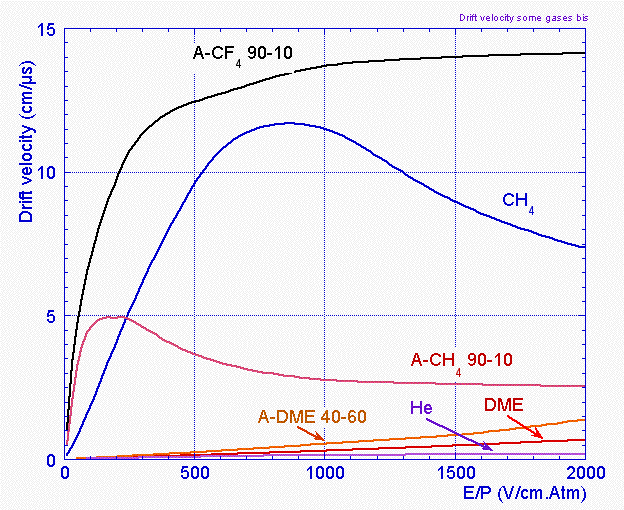
\includegraphics[width=0.6\textwidth]{immagini/mobilita.png}
\end{figure}
Se $\mu$ fosse esattamente costante dovremmo osservare delle rette, ma in pratica osserviamo tale andamento solo per bassi valori di campo elettrico. Tuttavia, dato che le condizioni in cui lavoriamo con i rivelatori a gas ricadono proprio in tale regione, possiamo tranquillamente supporre che la mobilità assuma un valore costante. Essa si esprime in $\rm m^2 \, atm \, V^{-1} \, s^{-1}$ e in generale assume valori molto più alti per gli elettroni piuttosto che per gli ioni, e ciò è legato alle masse in gioco. Ad esempio, in un gas come l'argon la mobilità degli elettroni è pari a $\mu_{\rm e}=2 \cdot 10^4$ mentre quella degli ioni è pari a $\mu_{\rm ioni}=1,5$. In conseguenza a queste profonde differenze nei valori di mobilità, quando si verifica una migrazione a seguito di un campo elettrico ci aspettiamo che gli elettroni si muovano molto velocemente mentre gli ioni abbiano una migrazione molto più lenta. Sempre in corrispondenza dell'argon, abbiamo che in esso $v_{\rm e}=3 \cdot 10^5 \; \rm cm/s$ e $v_{\rm ioni}=3 \cdot 10^2 \; \rm cm/s$, cioè differiscono di un fattore $10^3$. Nella seguente tabella possiamo vedere altri valori per altre miscele che confermano grossomodo questo fattore di differenza tra le due categorie di particelle:
\begin{center}
   \begin{tabular}{|c|c|c|}
     \hline
     &&\\[-0.4cm]
     Gas & $v_{\rm elettroni}$ (cm/s) & $v_{\rm ioni}$ (cm/s)\\
     \hline
     &&\\[-0.35cm]
     Ar & $3 \cdot 10^5$ & $3 \cdot 10^2$\\
     \hline
     &&\\[-0.35cm]
     He & $4 \cdot 10^5$ & $2 \cdot 10^3$\\
     \hline
     &&\\[-0.35cm]
     Ne & $10^6$ & $9 \cdot 10^2$\\
     \hline
     &&\\[-0.35cm]
     $\rm N_2$ & $4 \cdot 10^5$ & $5 \cdot 10^2$\\
     \hline
     &&\\[-0.35cm]
     $\rm H_2$ & $7 \cdot 10^5$ & $3 \cdot 10^3$\\
     \hline
     &&\\[-0.35cm]
     $\rm 95\% A + 5\% CO_2$ & $3.5 \cdot 10^6$ & $-$\\
     \hline
     &&\\[-0.35cm]
     $\rm CO_2$ & $10^5$ & $-$\\
     \hline
     &&\\[-0.35cm]
     $\rm CH_4$ & $1.5 \cdot 10^6$ & $-$\\
     \hline
   \end{tabular}
\end{center}
La conseguenza principale di questa enorme differenza nelle velocità tra ioni ed elettroni è che se volessimo raccogliere tutte le cariche prodotte dovremmo aspettare tempi elevati. Infatti gli elettroni dovranno arrivare fino all'anodo mentre gli ioni positivi fino al catodo\footnote{A patto di apparire prolissi, specifichiamo che per gli ioni positivi la velocità di drift è diretta come il campo elettrico, cioè dall'anodo (positivo) verso il catodo (negativo), mentre per gli elettroni ha direzione opposta.}, quindi devono percorrere uno spazio pari più o meno delle dimensioni del rivelatore stesso, e se consideriamo rivelatori della decina di centimetri possiamo stimare che per raccogliere le cariche dovute agli elettroni sono necessari tempi abbastanza brevi, dell'ordine dei microsecondi, mentre per raccogliere anche le cariche dovute agli elettroni dovremmo aspettare tempi molto più lunghi, dell'ordine dei millisecondi.

\newpage

\section{Struttura base di un rivelatore a gas}
Lo schema di principio di un rivelatore a gas include un recipiente a tenuta di gas con all'interno due
elettrodi per generare un campo elettrico e quindi una differenza di potenziale tra questi.

Un primo esempio di elettrodi che si possono adoperare è quello in cui essi sono piani e paralleli, come se costituissero un condensatore piano:

\begin{figure}[H]
   \centering
   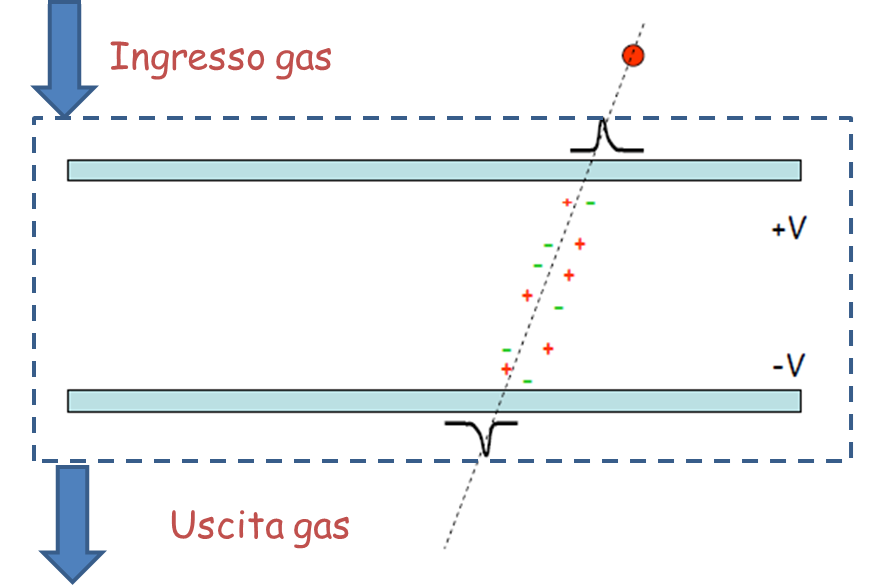
\includegraphics[width=0.6\textwidth]{immagini/modello_riv_gas_condensatore.png}
\end{figure}

Come vediamo in figura, al passaggio di una carica si genera ionizzazione e i prodotti della ionizzazione (gli elettroni e gli ioni) cominciano a migrare a seguito dell'effetto del campo elettrico creato dagli elettrodi.

Per quanto riguarda le caratteristiche del gas, esso si può trovare o in condizioni statiche, quindi viene inserito nella camera e sigillato, oppure in condizioni dinamiche, per cui si hanno dei flussi continui in quanto i rivelatori possiedono un ingresso e un'uscita del gas in maniera tale da avere sempre un ricircolo e quindi una miscela di gas sempre corrispondente alle percentuali che sono state fissate all'inizio. Quest'ultimo è il regime in cui lavorano soprattutto i rivelatori che non hanno una tenuta ottimale.

%\subsection{Misura del segnale}
\subsection{Formazione dell'impulso}
In generale possiamo schematizzare un rivelatore a gas come un condensatore, il quale viene polarizzato\footnote{Polarizzare un condensatore significa applicare una tensione ai suoi terminali in modo da stabilire una differenza di potenziale tra le sue armature. In particolare, si parla di polarizzazione quando il condensatore è polarizzato, cioè ha un lato che deve essere collegato al polo positivo e un lato che deve essere collegato al polo negativo dell'alimentazione.} attraverso una resistenza $R$ di valore molto elevato ($10^7-10^8 \; \Omega$).

\vspace{-0.1cm}

\begin{minipage}{0.395\textwidth}
   \begin{figure}[H]
      \centering
      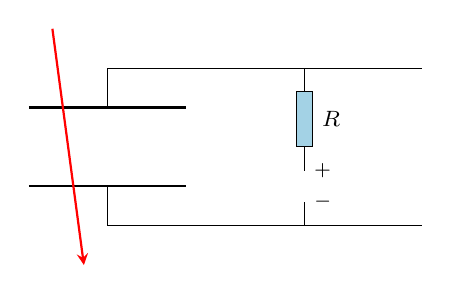
\begin{tikzpicture}
         %condensatore
         \draw[thick] (-1,0.5) -- (1,0.5);
         \draw[thick] (-1,-0.5) -- (1,-0.5);
         \draw (0,0.5) -- (0,1) -- (4,1);
         \draw (0,-0.5) -- (0,-1) -- (4,-1);
         %resistenza
         \draw (2.5,1) -- (2.5,-0.3) node[right] {\scriptsize$+$};
         \draw (2.5,-0.7) node[right] {\scriptsize$-$} -- (2.5,-1);
         \draw[fill=cyan!60!gray!50!] (2.4,0.7) -- (2.6,0.7) -- (2.6,0) node[midway, right] {\footnotesize$R$} -- (2.4,0) -- cycle;
         %segnale
         \draw[red,thick, -stealth] (-0.7,1.5) -- (-0.3,-1.5);
       \end{tikzpicture}
   \end{figure}
\end{minipage}
\begin{minipage}{0.6\textwidth}
   \vspace{0.5cm}Il motivo è che quando le cariche si avvicinano agli elettrodi (gli elettroni vanno verso l'anodo, gli ioni positivi verso il catodo), sugli elettrodi si genera una leggera variazione della tensione, proprio per il fatto che sono arrivate queste cariche, le quali quindi inducono una variazione nel valore di potenziale presente sugli elettrodi.
\end{minipage}

\vspace{0.1cm}

Se quindi gli elettrodi non fossero polarizzati, sarebbero destinati a scaricarsi velocemente. Dal momento che però gli elettrodi sono mantenuti a una differenza di potenziale costante attraverso un generatore di tensione, quello che succede è che la tensione viene subito riportata al valore nominale.

\begin{esempio}
   Come abbiamo detto, nel momento in cui passa una particella si producono delle cariche che generano una leggera variazione di tensione in queste piastre, ma grazie al collegamento con il generatore di tensione il potenziale viene immediatamente riportato al valore nominale. La velocità con cui ciò avviene dipende dalla resistenza del circuito, in quanto abbiamo sostanzialmente un circuito $RC$ e quindi la velocità del processo è stabilita dalla legge di carica di un condensatore nel caso in cui la carica iniziale non è nulla:
   \begin{equation*}
      V(t)=V_0 - (V_0 - \Delta V) e^{-\frac{t}{\tau}}
   \end{equation*}
   dove comanda il fattore $\tau=RC$, quindi più è grande $R$ più lenta sarà la risalita verso il valore nominale.\\
   Cerchiamo ora di capire quanto varia questa tensione tramite un esempio numerico. Supponiamo che gli elettrodi si trovino ad una differenza di potenziale $V_0=500 \; \rm V$ e che costituiscano un condensatore di capacità $C=50 \; \rm pF$. Immaginiamo poi che passi una particella di energia $5 \; \rm MeV$ che riesce a depositare tutta la sua energia all'interno del condensatore, quindi $E_{\rm dep}=5 \; \rm MeV$ e andiamo a valutare quanto vale la differenza di potenziale che si genera ai capi del condensatore a seguito della produzione di carica per ionizzazione.\\
   Innanzitutto calcoliamo la carica che viene prodotta e che viene raccolta da ciascun elettrodo. Per fare ciò basta calcolare il numero di coppie prodotte e moltiplicare queste per la carica dell'elettrone:
   \begin{equation*}
      Q=e\frac{E_{\rm dep}}{W}
   \end{equation*}
   Se adesso dividiamo questa carica per la capacità del condensatore otteniamo la differenza di potenziale che si genera a seguito dell'interazione: supponendo per semplicità $W=1$, avremo
   \begin{equation*}
      \Delta V
      =\frac{Q}{C}
      =e\frac{E_{\rm dep}}{WC}
      =0.5 \; \rm mV
   \end{equation*}
   Quello che quindi succede è che a seguito del passaggio di una particella si produce un segnale elettrico e di conseguenza una variazione del valore di tensione, che abbiamo trovato essere dell'ordine di mezzo mV. Capiamo quindi che sono segnali veramente piccoli da rivelare, per cui bisogna cercare di rallentare il più possibile la risalita verso il valore nominale di tensione. Ecco spiegato perché si adoperano valori di resistenze elevati.
\end{esempio}

%\vfill

%\subsection{Formazione dell'impulso}

Quando le cariche prodotte vengono raccolte, la tensione agli elettrodi diminuisce dal valore $V_0$ al valore $V_0 - ne/C$, per poi ritornare al valore $V_0$ con legge di carica
esponenziale avente velocità dipendente dalla costante di tempo $RC$.\footnote{Nelle slide la professoressa riporta questo grafico smussato. A livello teorico è giusto che ci sia un punto angoloso, ma come dice il Knoll: "In qualsiasi situazione reale, la radiazione incidente crea coppie di ioni su una gamma di posizioni all'interno della camera. Le discontinuità nette mostrate risultano quindi in qualche modo 'sfumate' nella forma dell'impulso risultante."}

\begin{figure}[H]
   \centering
   %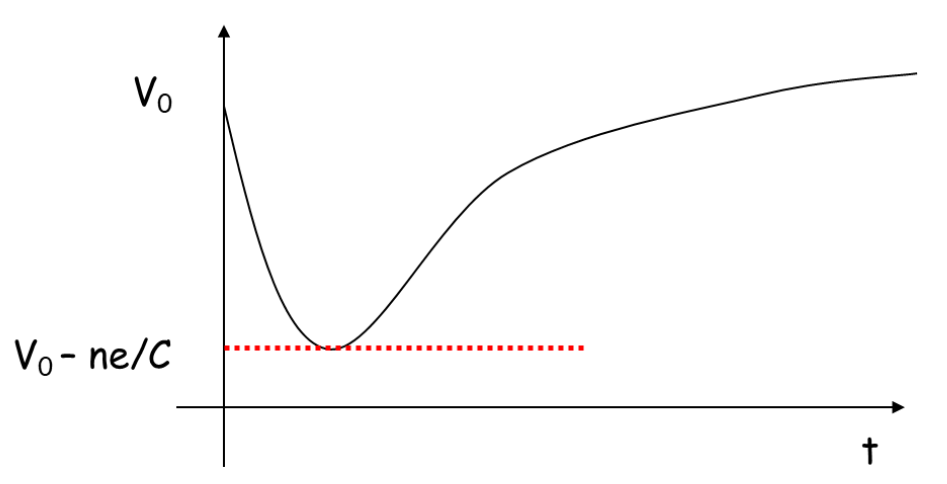
\includegraphics[width=0.6\textwidth]{immagini/impulso_rivelatori_a_gas.png}
   \begin{tikzpicture}
      %assi
      \draw[->] (0,0) -- (7,0) node[right] {$t$};
      \draw[->] (0,0) -- (0,4) node[above] {$V(t)$};
      \draw[red,dashed] (0,0.406) node[left,black] {$V_0 - ne/C$} -- (6.8,0.406);
      \node[left] at (0,3) {$V_0$};
      %grafico
      \draw[thick,teal!80!black] plot[domain=0:2,smooth] (\x, {3*exp(-\x)}) -- plot[domain=0:4.5,smooth] (\x+2, {3*(1 - exp(-\x)) + 0.406*exp(-\x)});
    \end{tikzpicture}
\end{figure}

Ragioniamo ora su che valori deve avere questa costante di tempo.

Se fosse $RC=\infty$, cioè se adoperassimo una resistenza eccessivamente grande, non torneremmo più al valore nominale e quindi la variazione si manterrebbe nel tempo:

\begin{figure}[H]
   \centering
   \begin{tikzpicture}
      %assi
      \draw[->] (0,0) -- (7,0) node[right] {$t$};
      \draw[->] (0,-3.5) -- (0,1) node[above] {$\Delta V(t)$};
      \draw[red,dashed] (0,-3) node[left,black] {$- ne/C$}-- (7,-3);
      %grafico
      \draw[thick,teal!60!black] plot[domain=0:6,smooth] (\x, {-3*(1 - exp(-\x) )}) node[above=0.2cm, black] {$RC=\infty$};
    \end{tikzpicture}
\end{figure}

Chiaramente questa non è una situazione che vogliamo, in quanto vogliamo che a un certo punto si ripristinino le condizioni di partenza in modo da poter essere pronti per una nuova rivelazione.

Facciamo allora un passo indietro: ricordiamo che la raccolta della carica avviene attraverso due fasi successive, perché dapprima avviene la raccolta degli elettroni che sono molto veloci e quindi arrivano subito all'anodo, ma poi abbiamo la migrazione degli ioni che è molto più lenta e quindi comporterà un'ulteriore parte di segnale che corrisponderà a tempi più lunghi. Siccome questo comporterebbe avere un rivelatore molto lento (cioè se volessimo raccogliere tutte le cariche, sia elettroni che ioni, dovremmo aspettare tempi lunghi proprio perché dobbiamo aspettare che gli ioni giungano al catodo), potremmo pensare di accontentarci del segnale prodotto dagli elettroni e quindi potremmo scegliere una costante di tempo tale che il segnale risalga dopo aver raccolto gli elettroni. In altre parole, il valore di $RC$ deve essere compreso tra il tempo minimo necessario a raccogliere il segnale dovuto agli elettroni, $t_{-}$, e il tempo minimo necessario a raccogliere gli ioni, $t_{+}$, cioè $t_{-} < RC < t_{+}$.

Il motivo per cui si trascura quello che fanno gli ioni è che altrimenti si avrebbero dei rivelatori particolarmente lenti. Infatti, nell'ambito della rivelazione parliamo di rivelatori lenti già quando abbiamo tempi dell'ordine dei microsecondi, che sono i tempi necessari per raccogliere gli elettroni, quindi se dovessimo arrivare ai millisecondi la situazione sarebbe ancora peggiore.

\begin{figure}[H]
   \centering
   \begin{tikzpicture}
      %assi
      \draw[->] (0,0) -- (7,0) node[right] {$t$};
      \draw[->] (0,-3.5) -- (0,1) node[above] {$\Delta V(t)$};
      \draw[red,dashed] (0,-3) node[left,black] {$- ne/C$}-- (7,-3);
      \node[left] at (0,-1.5) {$-\frac{1}{2} ne/C$};
      %grafico
      \draw[thick,teal!60!black,join=round] plot[domain=0:0.69314,smooth] (\x, {-3*(1 - exp(-\x) )}) -- plot[domain=0:4,smooth] (\x+0.69314, {3*(1 - 0.5*exp(-\x)) - 3});
      \draw[thick,teal!60!black,dashed] plot[domain=0.69314:6,smooth] (\x, {-3*(1 - exp(-\x) )}) node[above=0.2cm, black] {$RC=\infty$};
      \node at (3.1,-0.75) {$t_{-} < RC < t_{+}$};
    \end{tikzpicture}
\end{figure}

Poiché consideriamo soltanto il segnale che viene generato dalla raccolta degli elettroni, è chiaro che si avranno dei segnali ancora più piccoli in ampiezza, in quanto viene raccolta soltanto metà della carica disponibile; tuttavia ci accontentiamo di ciò perché tali segnali risultano più veloci.

\subsection{Il problema della posizione}
Un problema che può sorgere è legato al punto in cui si generano le cariche. Infatti il volume del rivelatore è un volume esteso e in base alla traiettoria che segue la particella queste cariche di ionizzazione potrebbero prodursi in diversi punti della camera.

Schematizziamo l'evento come segue: gli elettrodi si trovano a una distanza $d$ e supponiamo che la ionizzazione avvenga ad una distanza $x$ da un elettrodo, ad esempio quello inferiore:

\begin{figure}[H]
   \centering
   \begin{tikzpicture}
      \draw[thick, black!20!gray] (0,1.5) -- (6,1.5);
      \draw[thick, black!20!gray] (0,-1.5) -- (6,-1.5);
      \draw[thick,-stealth,shorten >= 0.3cm] (-1.5,-0.5) -- (0,-0.5);
      \draw[thick, dashed,red] (0,-0.5) -- (5,-0.5);
      \draw[<->] (6.3,1.5) -- (6.3,-0.5) node[midway, right] {$d-x$};
      \draw[<->] (6.3,-1.5) -- (6.3,-0.5) node[midway, right] {$x$};
      \node at (-1.4,0.5) {$\displaystyle V=\frac{ne}{C} \frac{x}{d}$};
   \end{tikzpicture}
\end{figure}

In base al valore di $x$, la raccolta del segnale e quindi la tensione che misuriamo ai capi delle armature potrebbe essere leggermente diversa. Il motivo è che le cariche dovranno percorrere uno spazio più o meno grande per arrivare all'anodo, impiegando quindi più o meno tempo. Siccome la costante di tempo, una volta scelta, è fissa, il segnale misurato sarà proporzionale allo spazio percorso, quindi più è grande questo più carica si può raccogliere. Ciò non costituisce un aspetto positivo per la raccolta, perché questo potrebbe portare a dei segnali di ampiezza veramente piccole.

Quello che normalmente si fa per cercare di evitare questo effetto è schermare gli ioni, in quanto il problema nasce dal fatto che scegliamo una costante di tempo opportuna per poter trascurare il segnale dovuto gli ioni.

Se scegliamo una costante di tempo che assicura la raccolta completa degli elettroni e permette di ignorare gli ioni, è possibile andare ad aggiungere una griglia in prossimità del catodo che viene detta \textit{griglia di Frisch} che va a schermare il catodo dall'arrivo degli ioni. Ciò permette di trascurare il segnale dovuto agli ioni e di scegliere una costante di tempo $RC$ anche un po più piccola, permettendo così di ricostruire tutta la carica prodotta indipendentemente dalla posizione in cui avviene l'interazione. 

\begin{approfondimento}[La forma del segnale]
   \footnotesize
   L'approfondimento che segue è sostanzialmente una traduzione di \S 5.VI.B "Pulse mode operation-Derivation of the pulse shape" del Knoll. Lo riporto perché spiega approfonditamente il perché i segnali abbiano quella forma.

   \vspace{0.2cm}L'analisi della forma dell'impulso prodotto dal flusso di cariche all'interno di una camera a ionizzazione con elettrodi a piastre parallele che sono separati da uno spazio piccolo rispetto alla lunghezza e alla larghezza delle piastre coinvolge una sola variabile: la posizione delle cariche nella dimensione perpendicolare alle piastre. È quindi istruttivo seguire una derivazione semplificata della forma dell'impulso che invoca argomenti basati solo sulla conservazione dell'energia. Questa derivazione fornisce risultati corretti ed evita la complessità matematica che potrebbe oscurare alcuni dei comportamenti fisici importanti nella determinazione delle caratteristiche dell'impulso di uscita atteso in queste condizioni.\\
   Nella derivazione che segue, assumiamo che venga applicato un campo elettrico sufficiente affinché la ricombinazione elettrone-ione sia trascurabile e che le cariche negative rimangano sotto forma di elettroni liberi. Per prima cosa, deriviamo un'espressione per la forma dell'impulso nel caso in cui la costante di tempo del circuito di raccolta sia molto più lunga dei tempi di raccolta di ioni ed elettroni.\\
   La forma dell'impulso dipende dalla configurazione del campo elettrico e dalla posizione in cui si formano le coppie di ioni rispetto alle superfici equipotenziali che caratterizzano la geometria del campo. Per semplificare l'analisi seguente, assumiamo che gli elettrodi della camera siano piastre parallele, per le quali le superfici equipotenziali sono piani uniformemente distanziati paralleli alle superfici degli elettrodi, e l'intensità costante del campo elettrico è data da
   \begin{equation*}
      E=\frac{V}{d}
   \end{equation*}
   dove $V$ è la tensione tra gli elettrodi della camera e $d$ è la loro distanza. Come ulteriore semplificazione, assumiamo che tutte le coppie di ioni si formino a una distanza uguale $x$ dall'elettrodo positivo, dove il potenziale elettrico è uguale a $Ex$. Questa situazione è illustrata nella figura seguente:
   \begin{figure}[H]
      \centering
      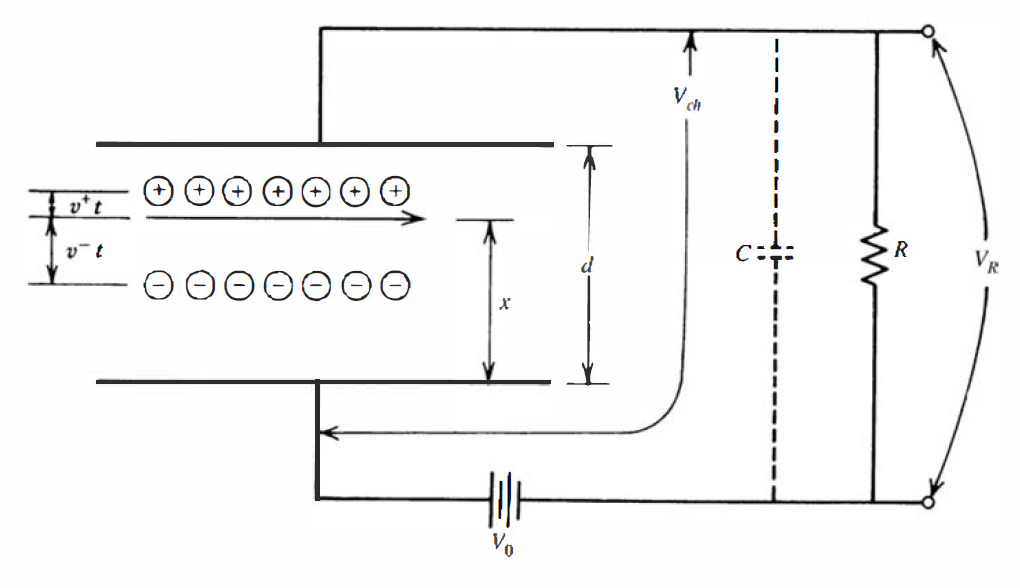
\includegraphics[width=0.6\textwidth]{immagini/circuito_forma_segnale.png}
   \end{figure}
   Poiché si assume che la costante di tempo del circuito esterno sia grande, non può fluire una corrente apprezzabile durante il tempo relativamente breve necessario per raccogliere le cariche all'interno della camera a ionizzazione. Pertanto, l'energia necessaria per spostare le cariche dal loro punto di origine deve provenire dall'energia inizialmente immagazzinata attraverso la capacità $C$, rappresentata dalla camera a ionizzazione. Questa energia è
   \begin{equation*}
      \mathcal{E}=\frac{1}{2}CV_0^2
   \end{equation*}
   dove $V_0$ è la tensione applicata.\\
   Dopo un tempo $t$, gli ioni avranno percorso una distanza $v_{+}t$ verso il catodo, dove $v_{+} $ è la velocità di deriva degli ioni. Allo stesso modo, gli elettroni avranno percorso una distanza $v_{-}t$ verso l'anodo. Entrambi questi movimenti rappresentano lo spostamento di carica verso una regione di potenziale elettrico più basso, e la differenza in energia potenziale viene assorbita nel gas attraverso le molteplici collisioni che i portatori di carica subiscono con le molecole di gas durante il loro movimento. Questa energia è uguale a $Q \Delta\phi$ sia per gli ioni che per gli elettroni, dove $Q$ è la carica totale data da $Q=n_0e$, dove $n_0$ è il numero di coppie di ioni originarie e $e$ è la carica elettronica, e $\Delta\phi$ è la differenza di potenziale elettrico, data dal prodotto del campo elettrico $E$ e della distanza percorsa verso l'elettrodo.\\
   Applichiamo la conservazione dell'energia, che può essere scritta come:
   \begin{gather*}
      \begin{array}{ccccccc}
         \rm Energia &  & \rm Energia &  & \rm Energia & & \rm Energia\\
         \rm immagazzinata & = & \rm assorbita & + & \rm assorbita & + & \rm immagazzinata\\
         \rm iniziale &  & \rm dagli \; ioni &  & \rm dagli \; elettroni &  & \rm finale\\[0.3cm]
         \frac{1}{2}CV_0^2 & = & n_0 e \mathcal{E} v_{+} t & + & n_0 e \mathcal{E} v_{-} t & + & \frac{1}{2}CV_{\rm Ch}^2
      \end{array}
      \\
      \frac{1}{2}C \bigl( V_0 - V_{\rm Ch} \bigr)^2
      =n_0 e \mathcal{E} \bigl( v_{+} + v_{-} \bigr) t
      \\
      \frac{1}{2}C \bigl( V_0 + V_{\rm Ch} \bigr)\bigl( V_0 - V_{\rm Ch} \bigr)
      =n_0 e \qty( \frac{V_{\rm Ch}}{d} ) \bigl( v_{+} + v_{-} \bigr) t
   \end{gather*}
   La tensione del segnale è misurata attraverso $R$ ed è denotata con $V_R$. Essa è quasi sempre piccola rispetto a $V_0$ ed è data da $V_R=V_0-V_{\rm Ch}$. Possiamo quindi fare le approssimazioni
   \begin{equation*}
      V_0 + V_{ch} \approx 2 V_0
      \qqtext{,}
      \frac{V_{\rm Ch}}{d} \approx \frac{V_0}{d}
   \end{equation*}
   Inserendo queste approssimazioni nell'equazione precedente otteniamo:
   \begin{gather*}
      \frac{1}{2}C(2V_0)V_R=n_0 e \qty( \frac{V_0}{d} ) \bigl( v_{+} + v_{-} \bigr) t
      \implies
      V_R=\frac{n_0 e}{C d} \bigl( v_{+} + v_{-} \bigr) t
   \end{gather*}
   Questo risultato descrive la porzione iniziale dell'impulso del segnale e prevede una crescita lineare con il tempo. È valido solo per il periodo in cui sia gli ioni che gli elettroni si stanno ancora muovendo all'interno della camera.\\
   Dopo un tempo $t_{-}=\frac{x}{v_{-}}$, gli elettroni raggiungono l'anodo. La loro deriva ha allora contribuito al massimo possibile alla tensione del segnale, e il secondo termine nell'espressione di $V_R$ diventa una costante pari al suo valore in $t_{-}$. Questo valore costante è $\frac{n_0 e v_{-} t_{-}}{Cd}$ o $\frac{n_0 e x}{Cd}$. Per il successivo periodo di tempo solo gli ioni si stanno ancora muovendo e $V_R$ assume la forma:
   \begin{equation*}
      V_R=\frac{n_0 e}{Cd} \bigl( v_{+} t + x\bigr)
   \end{equation*}
   Gli ioni raggiungono il catodo dopo un tempo $ t_+ = \frac{(d - x)}{v_{+}} $. A questo punto, la tensione del segnale non aumenta più avendo raggiunto infine il valore
   \begin{equation*}
      V_R=\frac{n_0 e}{Cd} \bigl[ (d - x) + x \bigr]
      =\frac{n_0 e}{C}
   \end{equation*}
   La forma dell'impulso nei vai intervalli è mostrata nella figura seguente:
   \begin{figure}[H]
      \centering
      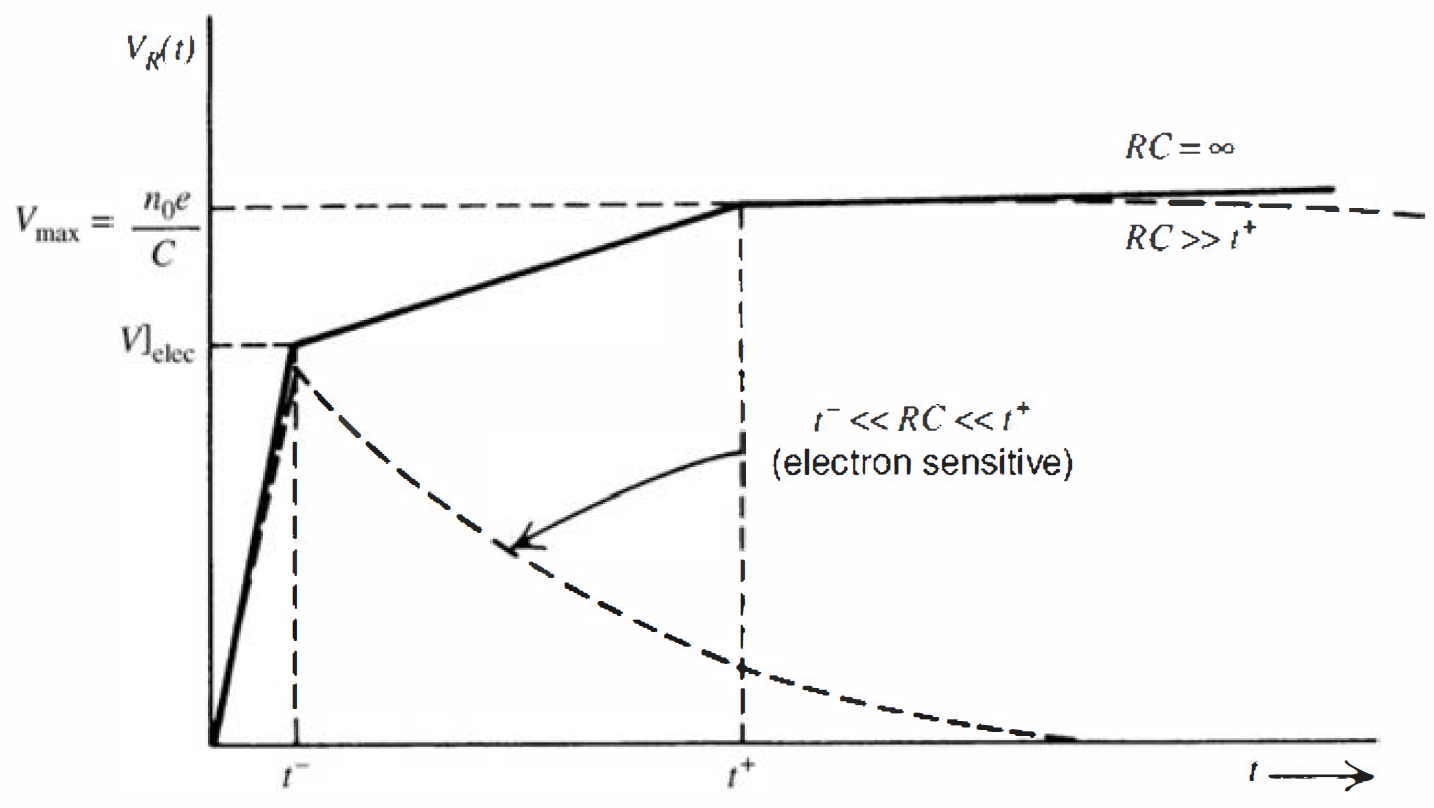
\includegraphics[width=0.7\textwidth]{immagini/forma_segnale_rivelatore_a_gas.png}
   \end{figure}
   Quando la costante di tempo del circuito di raccolta è molto grande, o $RC \gg t_{+}$, l'ampiezza massima dell'impulso del segnale è data da:
   \begin{equation*}
      V_{\text{max}}=\frac{n_0 e}{C}
   \end{equation*}
   e non dipende dalla posizione in cui le coppie di ioni sono state formate all'interno della camera. In queste condizioni, una misura dell'ampiezza dell'impulso $ V_{\text{max}} $ fornisce un'indicazione diretta del numero originario di coppie di ioni $n_0$ che hanno contribuito all'impulso.\\
   Nel funzionamento sensibile agli elettroni, tuttavia, la porzione dell'impulso derivata sopra, che corrisponde alla deriva degli ioni, è quasi completamente persa scegliendo una costante di tempo di raccolta molto più breve rispetto al tempo di raccolta degli ioni. L'impulso che rimane riflette quindi solo la deriva degli elettroni e avrà un'ampiezza data da
   \begin{equation*}
      V_{\text{elec}}=\frac{n_0 e}{C} \frac{x}{d}
   \end{equation*}
   La forma di questo impulso è anch'essa illustrata nella figura sopra. Solo la porzione a crescita rapida dell'impulso è preservata, e l'ampiezza adesso dipende dalla posizione $x$ in cui gli elettroni sono stati originariamente formati all'interno della camera.
\end{approfondimento}

\begin{approfondimento}[La griglia di Frisch]
   \footnotesize
   La dipendenza dell'ampiezza dell'impulso dalla posizione di interazione nelle camere a ionizzazione sensibili agli elettroni può essere eliminata attraverso l'uso di una configurazione illustrata nella figura seguente
   \begin{figure}[H]
      \centering
      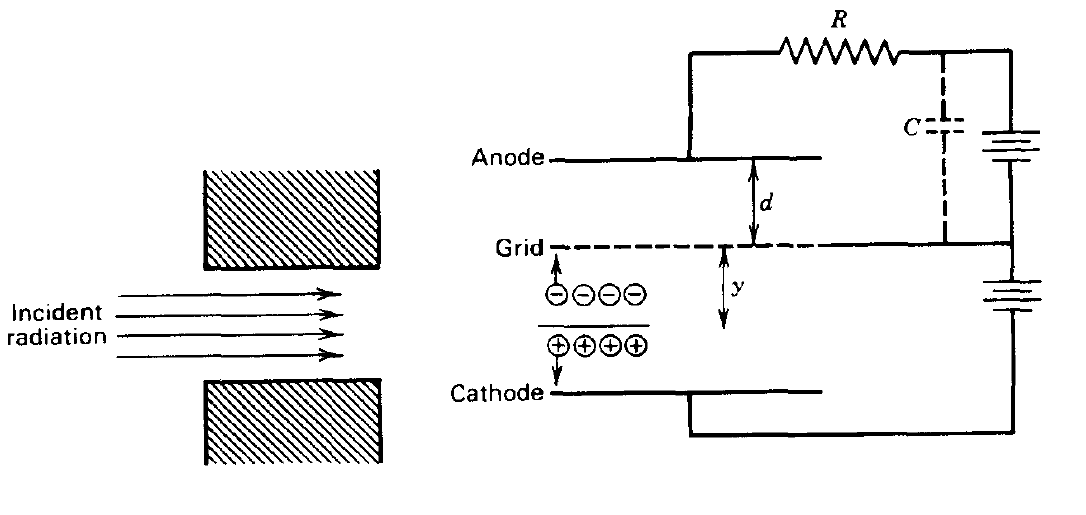
\includegraphics[width=0.7\textwidth]{immagini/griglia_di_frisch_1.png}
   \end{figure}
   In questo caso, il volume della camera a ionizzazione è diviso in due parti da una griglia di Frisch, chiamata così dal suo ideatore.\\
   Attraverso l'uso di una collimazione esterna o della posizione preferenziale della sorgente di radiazione, tutte le interazioni di radiazione sono confinate nel volume tra la griglia e il catodo della camera. Gli ioni positivi semplicemente si muoveranno da questo volume verso il catodo. La griglia è mantenuta a un potenziale intermedio tra i due elettrodi ed è realizzata in modo da essere il più trasparente possibile agli elettroni. Pertanto, gli elettroni sono inizialmente attratti dal volume di interazione verso la griglia. A causa della posizione del resistore di carico nel circuito, né la deriva verso il basso degli ioni né la deriva verso l'alto degli elettroni fino alla griglia producono alcuna tensione di segnale misurata. Tuttavia, una volta che gli elettroni attraversano la griglia dirigendosi verso l'anodo, la tensione griglia-anodo inizia a diminuire e una tensione di segnale inizia a svilupparsi attraverso il resistore. Per una costante di tempo del circuito grande rispetto al tempo di raccolta degli elettroni, il valore di tensione del segnale dipendente dal tempo attraverso il resistore è
   \begin{equation*}
      V_R=\frac{n_0 e}{Cd} v_{-} t
   \end{equation*}
   dove $d$ ora è la distanza tra la griglia e l'anodo. Questo aumento lineare continua fino a quando gli elettroni raggiungono l'anodo:
   \begin{figure}[H]
      \centering
      \begin{tikzpicture}
         \draw[->] (0,0) -- (9.5,0) node[right] {$t$};
         \draw[->] (0,0) -- (0,5) node[above] {$V_R(t)$};
         \draw[dashed,gray] (0,3) node[black,left] {$\displaystyle \frac{n_0 e}{C}$} -- (8,3);
         \draw[stealth-stealth] (0,4) -- (4.5,4) node[midway,above] {$y/v_{-}$};
         \draw[stealth-stealth] (4.5,4) -- (8,4) node[midway,above] {$d/v_{-}$};
         \draw[dashed,gray] (4.5,4.5) -- (4.5,-0.5);
         \draw[dashed,gray] (8,4.5) -- (8,-0.5);
         %grafico
         \draw[thick, red!70!black] (0,0) -- (4.5,0) node[black,midway, below=0.1cm] {
           $\begin{subarray}{c}
             \text{Gli elettroni si muovono}\\
             \text{verso la griglia}
           \end{subarray}$
         }
         -- (4.5,0) -- (8,3) -- (9.5,3);
         \node[black, below=0.1cm] at (6.25,0) {
           $\begin{subarray}{c}
             \text{Gli elettroni si muovono}\\
             \text{tra la griglia e l'anodo}
           \end{subarray}$
         };
       \end{tikzpicture}
   \end{figure}
   La tensione massima del segnale è quindi
   \begin{equation*}
      V_{\rm max}=\frac{n_0 e}{C}
   \end{equation*}
   che è identico a quella trovata nel caso in cui adoperiamo una costante di tempo $\tau \gg t_+$. Tuttavia, ora il segnale è dovuto solo alla deriva degli elettroni piuttosto che dal movimento sia degli elettroni che degli ioni positivi. L'aumento lento corrispondente alla deriva degli ioni è eliminato, e la costante di tempo del circuito può quindi essere impostata a un valore molto più breve tipico della modalità di funzionamento sensibile agli elettroni descritta nella sezione precedente. Poiché ogni elettrone attraversa la stessa differenza di potenziale e contribuisce ugualmente all'impulso di segnale, l'ampiezza dell'impulso è ora indipendente dalla posizione di formazione delle coppie di ioni originali ed è semplicemente proporzionale al numero totale di coppie di ioni formate lungo la traccia della particella incidente.
\end{approfondimento}

\vfill

\section{La moltiplicazione}

Un'ultimo aspetto da considerare in un rivelatore a gas è la moltiplicazione. La moltiplicazione è una conseguenza dell'aumento del campo elettrico all'interno del gas fino a un valore sufficientemente elevato (si parla di diversi kV/cm). Infatti, per valori bassi del campo, gli elettroni e gli ioni creati dalla radiazione incidente si limitano a migrare verso i rispettivi elettrodi di raccolta; tuttavia, per valori molto elevati del campo elettrico, gli elettroni acquisiscono una velocità estremamente elevata tanto che possono avere un'energia cinetica così grande da poter innescare ulteriori ionizzazioni, che sono delle ionizzazioni secondarie con cui si produrranno ulteriori coppie elettrone-ione.

\subsection{Moltiplicazione a valanga}
L'elettrone liberato da questo processo di ionizzazione secondaria verrà anch'esso accelerato dal campo elettrico. Durante la sua successiva deriva, subisce collisioni con altre molecole di gas neutro e può quindi creare ulteriori ionizzazioni. Il processo di moltiplicazione del gas assume quindi la forma di una cascata, nota come \textit{valanga di Townsend}, in cui ciascun elettrone libero creato in una collisione può potenzialmente creare più elettroni liberi tramite lo stesso processo.

\comment{\begin{figure}[H]
   \centering
   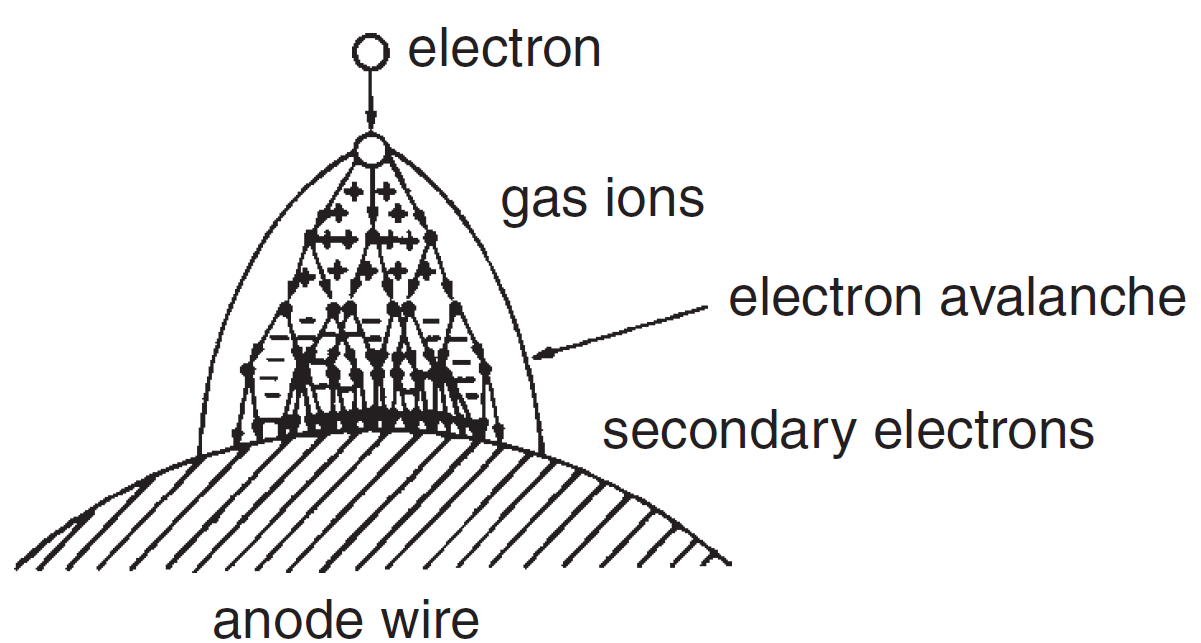
\includegraphics[width=0.6\textwidth]{immagini/valanga_ionizzazione_secondaria.png}
\end{figure}}

Se $\lambda$ è il libero cammino medio dell'elettrone per una collisione ionizzante secondaria, allora $\alpha=\frac{1}{\lambda}$ rappresenta il numero medio di coppie create per unità di percorso\footnote{Il Leo dice che tale costante corrisponde alla probabilità di ionizzazione per unità di lunghezza del cammino. Non capendo chi abbia ragione, riporto quanto detto dalla professoressa, che è anche ciò che si trova nella maggior parte dei testi.}. Questo è meglio conosciuto come il primo coefficiente di Townsend.

Se ci sono $n$ elettroni, allora in un cammino $\dd{x}$ verrà creato un numero di nuovi elettroni dato da
\begin{equation*}
   \dd{n}=n\alpha\dd{x}
\end{equation*}
Integrando, si ottiene il numero totale di elettroni creati in un cammino $x$ avendo $n_0$ elettroni iniziali (ottenuti dalla ionizzazione primaria):
\begin{equation*}
   n=n_0e^{\alpha x}
\end{equation*}
A partire da tale relazione è possibile definire il fattore di moltiplicazione o guadagno $M$, che rappresenta il numero di coppie create rispetto al numero di coppie prodotte per ionizzazione primaria:
\begin{equation*}
   M=\frac{n}{n_0}=e^{\alpha x}
\end{equation*}
\comment{\begin{approfondimento}[Il primo coefficiente di Townsend]
   \footnotesize
   Il primo coefficiente di Townsend $\alpha$ dipende dall'intensità del campo elettrico e dunque dalla posizione $x$ all'interno della camera a gas. In generale dunque il numero di particelle sarà dato da
   \begin{equation*}
      n(x)=n_0 \exp{ \int_{r_k}^{r_i} \alpha(x) \dd{x}}
   \end{equation*}
\end{approfondimento}}

Sostanzialmente, grazie a questi meccanismi di produzione a valanga possiamo produrre un numero di coppie molto elevato a partire da una singola prima ionizzazione. Ciò costituisce un vantaggio, perché avere più carica comporta un segnale più intenso dunque avente ampiezza maggiore.

C'è tuttavia un limite nei valori che fisicamente $M$ può assumere, perché superato questo si potrebbe produrre un danneggiamento del rivelatore in quanto cominciano a innescarsi delle scariche e delle valanghe incontrollate. Tale condizione è detta regime di breakdown, in cui si giunge se si supera il limite di breakdown, ovvero se il fattore di guadagno $M$ supera il valore di $10^8$. Tale limite è detto condizione di Raether.

\subsection{Sviluppo della valanga}

Lo sviluppo della valanga dipende dalle diverse velocità di deriva di elettroni e ioni. A causa della grande mobilità degli elettroni rispetto agli ioni positivi, la valanga assume la forma di una goccia avente sul fronte gli elettroni e sulla coda gli ioni.

\begin{minipage}{0.5\textwidth}
   \begin{figure}[H]
      \centering
      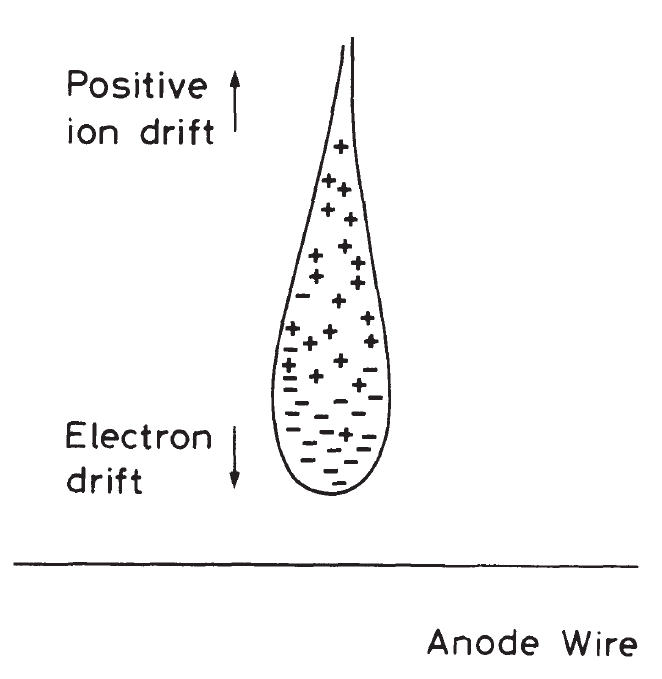
\includegraphics[width=0.9\textwidth]{immagini/forma_valanga_1.png}
   \end{figure}
\end{minipage}
\begin{minipage}{0.5\textwidth}
   \begin{figure}[H]
      \centering
      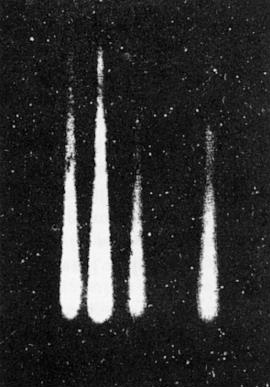
\includegraphics[width=0.65\textwidth]{immagini/forma_valanga_2.png}
   \end{figure}
\end{minipage}

\section{Regimi di lavoro dei rivelatori a gas}

Analizziamo ora le diverse regioni di funzionamento dei rivelatori a gas. Osserviamo il seguente grafico, dove sull'asse delle ascisse è riportata la tensione applicata tra gli elettrodi del rivelatore mentre sulle ordinate la carica raccolta dagli elettrodi:

\begin{figure}[H]
   \centering
   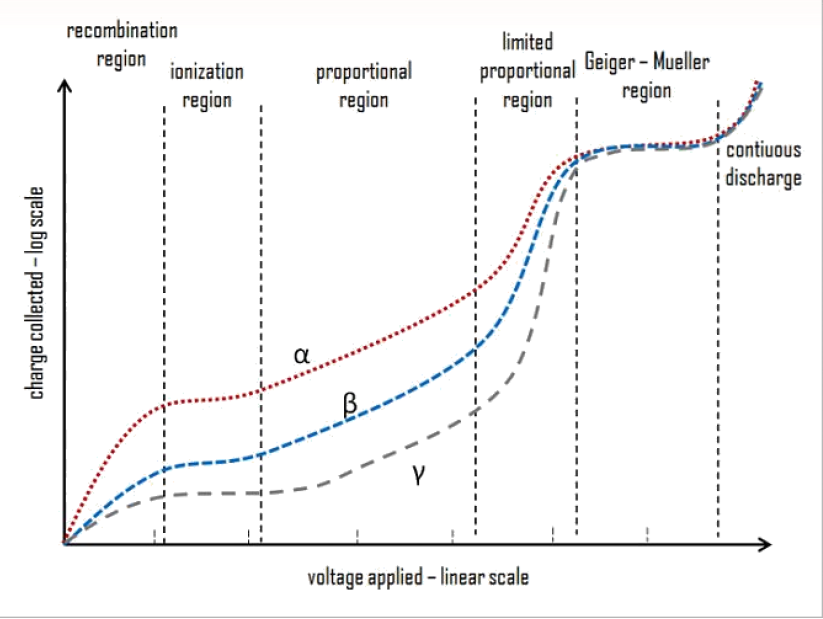
\includegraphics[width=0.85\textwidth]{immagini/regimi_rivelatori_a_gas.png}
\end{figure}

A seconda del valore di tensione applicata, dunque in base all'intensità del campo elettrico, si individuano diverse regioni:

\begin{itemize}[leftmargin=0.5cm]
   \item \textit{Regione di ricombinazione}: Quando le tensioni applicate sono abbastanza basse, quello che avviene quando passa una particella è che si producono le coppie elettrone-ione e queste tendono a migrare, ma poiché il campo elettrico non è molto intenso continuano a prevalere i processi di ricombinazione, per cui non riusciamo a raccogliere tutte le coppie prodotte in quanto una parte viene persa a causa dei fenomeni di ricombinazione;
   \item \textit{Regione di ionizzazione}: Man mano che aumenta la tensione, l'effetto di ricombinazione diventa via via sempre meno importante perché con la tensione aumenta la probabilità che la carica riesca a migrare fino all'elettrodo e quindi il segnale venga raccolto. Il segnale raccolto aumenterà fino a raggiungere un "pianerottolo", il quale fisicamente rappresenta il fatto che stiamo raccogliendo tutte le cariche che sono state prodotte, quindi anche aumentando la tensione il segnale non aumenterà in maniera sensibile. Questa regione di pianerottolo è la regione in cui funzionano le cosiddette camere a ionizzazione, le quali sono dei rivelatori che lavorano in un regime di tensione tale che si raccolgono tutte le cariche prodotte dalla prima ionizzazione;
   \item \textit{Regione proporzionale}: Continuando ad aumentare la tensione cominciano ad innescarsi i processi di produzione a valanga, quindi i campi elettrici diventano così intensi che gli elettroni prodotti dalla ionizzazione primaria possono innescare delle ionizzazioni secondarie e così via. Ci aspettiamo allora che il segnale cominci ad aumentare e quindi il numero di cariche raccolte; in particolare queste aumenteranno seguendo la legge esponenziale vista poc'anzi. In questa regione la ionizzazione secondaria è ancora strettamente dipendente
   da quella primaria. Infatti, anche se abbiamo una produzione a valanga di cariche, il numero di cariche prodotte rimane proporzionale all'energia depositata, quindi se siamo in grado di misurare quante cariche sono prodotte possiamo ancora avere l'informazione sull'energia che è stata depositata nel rivelatore. In tale regione funzionano i cosiddetti contatori proporzionali;
   \item \textit{Regione di proporzionalità limitata}: Se andiamo oltre incontriamo una prima regione di proporzionalità limitata in cui la carica prodotta è così grande che gli ioni vanno a modificare il campo elettrico generato dagli elettrodi. Viene dunque perturbata la proporzionalità che caratterizzava la zona precedente, per cui tale regione non viene normalmente adoperata per la rivelazione;
   \item \textit{Regione Geiger-Mueller}: Se aumentiamo ancora la tensione arriviamo a un secondo pianerottolo, che è il cosiddetto pianerottolo Geiger, in cui nuovamente abbiamo un segnale che è indipendente dalla tensione di lavoro. Il motivo è che siamo arrivati in una regione in cui cominciano a innescarsi delle valanghe in maniera incontrollata. A differenza della regione proporzionale dove ogni elettrone può innescare una nuova valanga, qui comincianono a innescarsi delle valanghe lungo l'anodo che vengono generate da fotoni emessi dalla diseccitazione degli atomi che compongono il gas, quindi incominciano a generarsi delle cariche in modo incontrollato e soprattutto il segnale che si ha in uscita, dunque il numero di cariche che misuriamo alla fine, diventa indipendente da quante cariche sono state prodotte dalla prima ionizzazione, quindi dall'energia che è stata depositata. In altre parole, il segnale in uscita non dà più alcuna informazione sull'energia depositata nel rivelatore. Nonostante sembri una regione meno interessante perché il segnale non ci fornisce informazioni sull'energia depositata, possiamo comunque sapere se è passata o meno una particella. Ecco perché in questa regione funzionano i contatori, rivelatori che permettono solamente di contare quante particelle sono passate senza fornire indicazioni sull'energia. Tra questi contatori abbiamo il contatore Geiger;
   \item \textit{Regione di scarica continua}: Oltre il secondo pianerottolo si va incontro ad una regione da evitare, perché a causa delle continue scariche si potrebbero verificare dei danneggiamenti del rivelatore.
\end{itemize}

Dall'analisi di questo grafico individuiamo tre tipologie di rivelatore a gas: camere a ionizzazione, camere proporzionali e rivelatori Geiger.

Inoltre il grafico presenta tre diverse curve al variare del tipo di particella all'interno del rivelatore al gas: una è relativa alle particella $\alpha$, una alle particelle $\beta$ e una ai $\gamma$. Tali curve mostrano qual è il segnale rilasciato a parità di tensione in base al tipo di radiazione. Notiamo che per i $\gamma$ la carica prodotta è più bassa in generale, mentre per le $alpha$ e le $\beta$ le differenze dipendono dallo stopping power di queste particelle all'interno del gas. Al di là dell dell'ordine con cui si presentano queste curve, la cosa che ci interessa di più è osservare che le curve sono ben distanziate finché lavoriamo nella regione delle camera a ionizzazione o in quella dei contatori proporzionali, ma poi si unificano. In particolare, in corrispondenza del contatore Geiger non c'è più alcuna distinzione, quindi indipendentemente dal tipo di particella e dall'energia che è stata depositata all'interno del rivelatore il segnale in uscita è sempre lo stesso. Ciò mostra come i contatori sono dei rivelatori basilari, che non danno altre informazioni se non il fatto che è passata una particella.

\section{Geometrie dei rivelatori a gas}

Il campo elettrico che si genera all'interno del rivelatore dipende dalla geometria del rivelatore. Sono possibili diverse configurazioni geometriche, a seconda delle dimensioni, del regime in cui i rivelatori devono operare e delle performance richieste.

\subsection{Geometria piana}
Una geometria molto semplice è quella costituita da due elettrodi a facce piane e parallele. Un rivelatore di questo tipo è equivalente ad un condensatore a facce piane e parallele distanti $d$ tra loro. Il campo elettrico che si genera nella regione compresa tra i due elettrodi è uniforme e vale

\begin{equation*}
   E=\frac{V}{d}
\end{equation*}

Questo tipo di geometria viene normalmente adoperata nelle camere a ionizzazione, quindi in una regione dove la tensione non è molto elevata, dunque non ci aspettiamo campi elettrici particolarmente intensi. Infatti i segnali che si producono in questo tipo di rivelatori sono segnali deboli rispetto alla tensione applicata alle armature.

\subsection{La geometrica cilindrica}
Se volessimo ottenere dei campi elettrici più intensi mantenendo la geometria piana, dovremmo aumentare la tensione $V$ o diminuire la distanza $d$. Tuttavia facendo ciò si potrebbe arrivare a superare la rigidità dielettrica del gas, giungendo dunque alla condizione di scarica, che è ovviamente una condizione da evitare.

Per produrre campi elettrici più intensi nella regione di rivelazione basta adoperare la geometria cilindrica:

\begin{figure}[H]
   \centering
   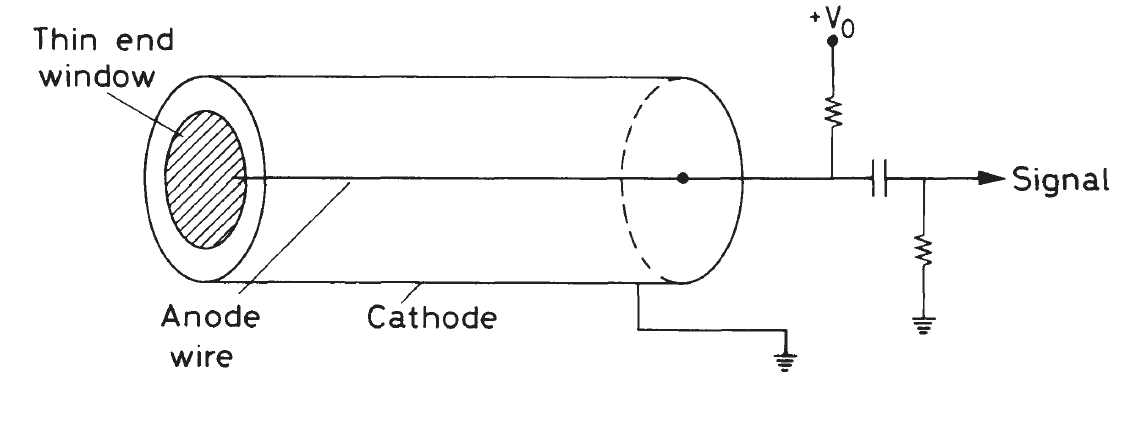
\includegraphics[width=0.75\textwidth]{immagini/geometria_cilindrica.png}
\end{figure}

Nella geometria cilindrica un elettrodo è costituito dal cilindro esterno, mentre l'altro da un filo disposto lungo l'asse del cilindro. Ovviamente il filo non è di dimensioni infinitesime, ma avrà anche esso un valore del raggio. Tra i due elettrodi, cioè quindi tra il cilindro esterno e il filo interno, viene creato una differenza di potenziale. Come possiamo vedere dalla figura, il cilindro esterno è collegato a massa mentre il filo interno è posto a un potenziale $V_0$, quindi il filo rappresenta l'anodo e il cilindro esterno il catodo.

Il principio di funzionamento è esattamente lo stesso: quando passa una particella, essa produce ionizzazione primaria, solo che stavolta abbiamo dei campi elettrici molto intensi e quindi si generano delle valanghe. \E addirittura possibile lavorare nella modalità Geiger, dove le valanghe sono incontrollate e il segnale in uscita è indipendente dalla particella e dall'energia depositata.

\begin{esempio}[Il campo elettrico della geometria cilindrica]
   Il motivo per cui il campo elettrico relativo a tale geometria è molto intenso deriva dalla forma funzionale di questo. Richiamiamo brevemente i passaggi necessari per giungere a tale espressione.

   Dal teorema di Gauss si ha che su una superficie Gaussiana cilindrica di raggio $r$ il flusso del campo elettrico è dato da
   \begin{equation*}
      \Phi
      =\int_{S} \vb{E} \vdot \dd{\vb{S}}
      =E2\pi r L
      =\frac{|Q|}{\varepsilon}
      \implies
      E(r)=\frac{|Q|}{2\pi\varepsilon L} \frac{1}{r}
   \end{equation*}
   in virtù della simmetria radiale del sistema. D'altro canto il sistema costituisce sostanzialmente un condensatore, dunque è valida la relazione
   \begin{equation*}
      \frac{|Q|}{\varepsilon}
      =\frac{C \Delta V}{\varepsilon}
   \end{equation*}
   Determiniamo allora $\Delta V$: detto $a$ il raggio del filo e $b$ il raggio del cilindro, si ha
   \begin{gather*}
      \Delta V
      =-\int_{a}^{b} \vb{E} \vdot \dd{\vb{r}}
      =-\int_{a}^{b} E \dd{r}
      =-\frac{|Q|}{2\pi\varepsilon L} \int_{a}^{b} \frac{1}{r} \dd{r}
      =-\frac{|Q|}{2\pi\varepsilon L} \ln\qty(\frac{a}{b})
      \\[0.2cm]
      \implies
      \frac{|Q|}{\varepsilon}
      =\frac{2\pi L \Delta V}{\ln\qty(\frac{b}{a})}
      \equiv \frac{2\pi L V_0}{\ln\qty(\frac{b}{a})}
   \end{gather*}
   in quanto nel nostro caso $\Delta V=V_0$. Andando a sostituire troviamo che
   \begin{equation*}
      E(r)=\frac{V_0}{r \ln\qty(\frac{b}{a})}
   \end{equation*}
   Il fatto che abbia un andamento del tipo $\frac{1}{r}$ fa sì che in prossimità dell'anodo si possano raggiungere valori di campo elettrico particolarmente intensi, addirittura per $r=0$ diventerebbe infinito. Inoltre esso dipende dalle caratteristiche geometriche del cilindro, in particolare dal raggio interno e da quello esterno.\\
   Vediamo un esempio numerico. Supponiamo che l'anodo abbia un raggio $a=0,01 \; \rm cm$ e il cilindro esterno abbia raggio $b=1 \; \rm cm$; applicando una differenza di potenziale $V=1 \; \rm kV$, in prossimità dell'anodo il campo elettrico raggiunge il valore di circa $21 \; \rm kV/cm$, che è molto più elevato rispetto ai valori che possiamo ottenere con la geometria a facce piane parallele, dove per ottenere lo stesso valore di campo elettrico dovremmo applicare, supponendo che le piastre siano distanti tra loro $d=1 \; \rm cm$, una differenza di potenziale di ben $21 \; \rm kV$.\\
   Il segnale che si genera è di conseguenza molto elevato, anche dell'ordine del Volt. Ricordiamo che questo va confrontato con la differenza di potenziale che si adopera tra gli elettrodi.
\end{esempio}

\subsection{Il contatore Geiger}

La geometria cilindrica è tipicamente adoperata in un contatore Geiger.

In questo tipo di rivelatori, al passaggio di una particella si producono delle scariche a valanga, con il risultato di un impulso molto elevato (dell'ordine dei Volt). Il segnale è indipendente dalla ionizzazione primaria, dunque dal tipo di particella e dall'energia di questa. Fornisce quindi solo un conteggio delle particelle.

Vediamo schematicamente cosa avviene:
\begin{figure}[H]
   \centering
   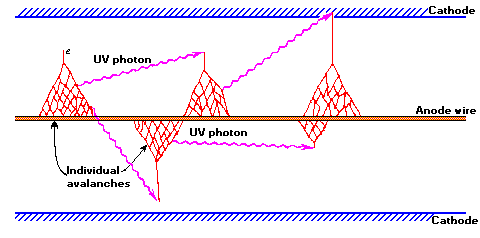
\includegraphics[width=0.7\textwidth]{immagini/contatore_geiger_valanghe.png}
\end{figure}
L'elettrone prodotto dalla ionizzazione primaria viene accelerato a causa del campo elettrico e riesce a produrre a sua volta ionizzazioni secondarie, dando luogo ad una valanga. Notiamo che lungo l'anodo ci sono tantissime altre valanghe che in realtà non derivano da un elettrone di ionizzazione primaria, bensì dai fotoni che vengono emessi a seguito della diseccitazione delle molecole. Sebbene siano quindi in qualche modo correlati alla prima valanga, perdiamo completamente la proporzionalità che caratterizzava la prima regione di lavoro dei rivelatori, ossia la regione di ionizzazione. Infatti il contatore Geiger lavora nella regione che prende il nome di "pianerottolo Geiger" che in realtà ha una leggera pendenza dell'ordine del $2-3\%/ \rm V$, cioè il segnale che ogni volta misuriamo può variare del $2-3\%$ per unità di tensione. %cento che non è tantissimo ovviamente però è un piccolo aumento
\begin{figure}[H]
   \centering
   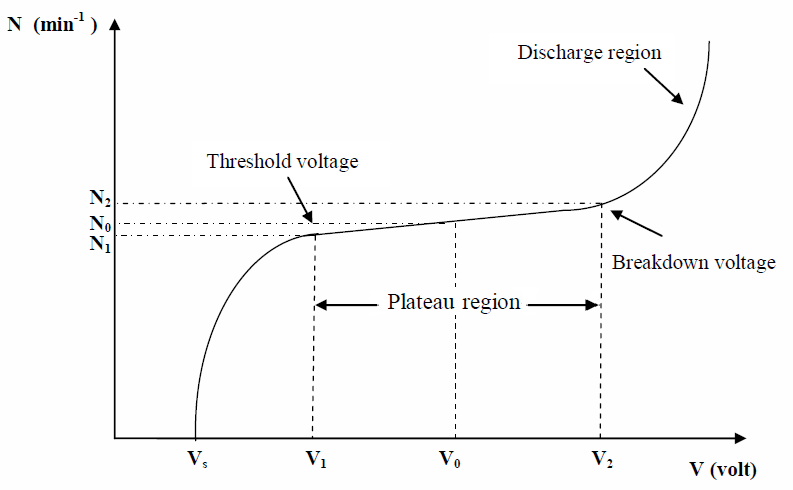
\includegraphics[width=0.7\textwidth]{immagini/Geiger_plateau.png}
\end{figure}
Quello che si fa quando si lavora con un contatore Geiger è cercare di capire la tensione di lavoro ottimale, quindi a quale valore di differenza di potenziale bisogna porre gli elettrodi del contatore Geiger per lavorare all'incirca al centro del pianerottolo, perché bisogna evitare di lavorare in prossimità delle estremità del pianerottolo altrimenti si rischia di entrare in regimi di lavoro che vogliamo evitare. Infatti a destra abbiamo la regione di breakdown, dove si innescano delle scariche tra gli elettrodi ed è una regione in cui il rivelatore può anche danneggiarsi, mentre a sinistra abbiamo la regione di proporzionalità limitata, che è una regione che non ci interessa ai fini della rivelazione. Quindi bisogna aumentare man mano la tensione per verificare quando si raggiunge il pianerottolo e cercare di adoperare una tensione di lavoro in prossimità del centro del pianerottolo.

\vspace{0.2cm}Vediamo ora cosa può rivelare un contatore Geiger (ma ciò vale in generale anche per altri rivelatori a gas):

\begin{itemize}[leftmargin=0.5cm]
   \item \textit{Particelle cariche}: \E chiaro che le particelle cariche vengano rivelate in quanto queste ionizzano la materia. L'unico fattore a cui bisogna stare attenti riguarda l'ingresso all'interno del rivelatore, perché il rivelatore è un recipiente chiuso ermeticamente per contenere il gas, quindi affinché le particelle vengano rivelate devono necessariamente attraversare le pareti del rivelatore. Finché abbiamo a che fare con elettroni, i quali hanno un potere penetrante abbastanza discreto, se si realizzano delle finestre di ingresso sottili, che nella pratica significa che una delle pareti del contatore Geiger viene realizzata con un materiale avente un basso stopping power, magari particolarmente sottili e/o con densità bassa\footnote{Per dare un'idea quantitativa, con una densità superficiale pari a $4 \; \rm mg/cm^2$, il coefficiente di trasmissione $T$ è dell'85\%, mentre con una densità di $30 \; \rm mg/cm^2$ $T$ scende all'85\%.}, allora l'elettrone perde una piccola parte della sua energia ma riesce comunque a penetrare all'interno del rivelatore. Nel caso del contatore Geiger l'efficienza di rivelazione (che ricordiamo rappresentare il rapporto tra il numero di particelle rivelate e il numero di particelle incidenti) per gli elettroni è del 100\%, cioè tutti gli elettroni che incidono sul contatore Geiger vengono rivelati;
   \item \textit{Raggi }$\gamma$: I raggi $\gamma$ interagiscono con la materia attraverso vari meccanismi, ma non sono direttamente ionizzanti. Possono invece causare effetti come l'effetto fotoelettrico, l'effetto Compton e la produzione di coppie. Sono quindi i prodotti carichi di queste interazioni a poter ionizzare il gas. Ad esempio, se si verifica l'effetto fotoelettrico, l'elettrone emesso sarà in grado di ionizzare il gas.\\
   Per rivelare un $\gamma$, è essenziale che avvenga un'interazione. È molto probabile che il $\gamma$ interagisca con le pareti del contenitore, poiché queste hanno una densità e un numero atomico $Z$ elevati. Al contrario, è meno probabile che il $\gamma$ interagisca direttamente con il gas, a causa dei bassi valori di densità e $Z$ di questo. Di conseguenza, l'efficienza nel rivelare i raggi $\gamma$ è molto bassa, intorno all'$1-2\%$, poiché il $\gamma$ deve interagire con le pareti del materiale, e i prodotti di questa interazione devono poi generare un segnale nel contatore Geiger;
   \comment{I raggi $\gamma$ interagiscono attraverso meccanismi diversi: essi non ionizzano la materia, quello che possono fare è produrre effetto fotoelettrico, effetto Compton e produzione di coppie. Quindi eventualmente sono i prodotti carichi di queste interazioni che possono ionizzare il gas, quindi se ad esempio avviene effetto fotoelettrico sarà l'elettrone emesso per effetto fotoelettrico a poter ionizzare il gas.
   \begin{figure}[H]
      \centering
      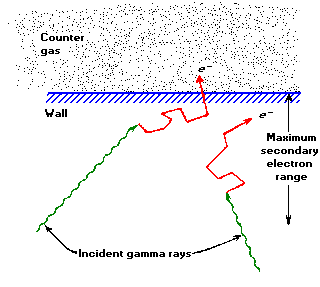
\includegraphics[width=0.5\textwidth]{immagini/interazione_gamma_gas.png}
   \end{figure}
   Quindi, affinché il $\gamma$ venga rivelato, è necessario che interagisca. \E molto probabile che il $\gamma$ possa interagire con le pareti perché le pareti hanno una densità numero atomico $Z$ elevato, mentre è più difficile che il $\gamma$ interagisca con il gas stesso sia per una questione di densità sia per una questione del valore di $Z$ del gas. In conseguenza a ciò l'efficienza nel caso del raggi $\gamma$ è quasi nulla, intorno all'$1-2\%$, perché il $\gamma$ deve interagire con le pareti del materiale e i prodotti di questa interazione devono poi produrre un segnale del contatore Geiger;}
   \item \textit{Muoni cosmici}: I muoni hanno un elevato potere penetrante, pertanto riescono ad attraversare tranquillamente le pareti del recipiente senza essere schermati o assorbiti, dunque per questa tipologia di particelle l'efficienza è del 100\%.
\end{itemize}

Restano fuori da questo schema le particelle $\alpha$ e più in generale le particelle cariche pesanti. Queste percorrono spessori di materiale solido veramente piccoli per poi venire fermate, ad esempio bastano circa $50 \; \rm \mu m$ di silicio per arrestare una particella $\alpha$ da $1 \; \rm MeV$. Capiamo quindi che una qualsiasi parete arresterebbe le particelle $\alpha$ o nella migliore delle ipotesi farebbe perdere loro gran parte dell'energia. Ne segue che è veramente difficile misurare particelle $\alpha$ con il contatore Geiger.

\section{Rivelatori a gas moderni}

Affrontiamo adesso brevemente alcuni rivelatori a gas un po' più moderni. Infatti i rivelatori di cui abbiamo parlato finora sono rivelatori storici, in quanto sono stati i primi ad essere stati sviluppati e che ormai non si usano più nel campo della ricerca. In particolare, i contatori Geiger vengono adoperati più per scopi didattici-dimostrativi perché sono dei rivelatori molto semplici, mentre i contatori proporzionali o le camere a ionizzazione sono per lo più utilizzate in ambito medico.

\subsection{MWPC (Multiwire Proportional Chambers)}

Una prima tipologia di rivelatori a gas più moderna sono le cosiddette Multiwire Proportional Chambers, anche dette camere a fili. Queste sono state sviluppate intorno agli anni '70 e, sostanzialmente, si comportano come un insieme di contatori proporzionali. In camere di questo tipo abbiamo due superfici piane, una sopra e una sotto, costituenti dei catodi; al centro della camera invece abbiamo diversi fili che rappresentano gli anodi:

\begin{minipage}{0.49\textwidth}
   \begin{figure}[H]
      \centering
      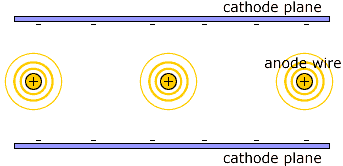
\includegraphics[width=\textwidth]{immagini/MWPC_1.png}
   \end{figure}
\end{minipage}
\hfill
\begin{minipage}{0.49\textwidth}
   \begin{figure}[H]
      \centering
      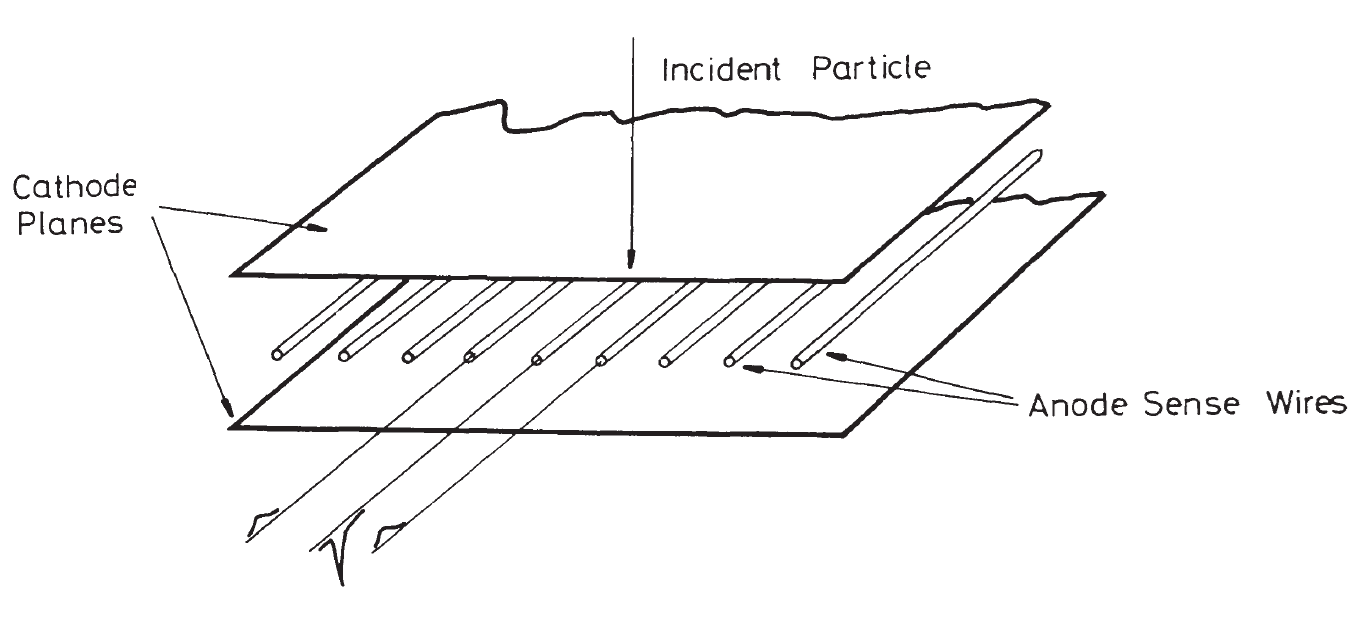
\includegraphics[width=\textwidth]{immagini/MWPC_2.png}
   \end{figure}
\end{minipage}

\vspace{0.4cm}Il fenomeno che avviene è lo stesso che si verifica all'interno di un qualsiasi rivelatore a gas: una particella entra, produce delle coppie elettrone-ione positivo per ionizzazione e gli elettroni viaggiano verso l'anodo, mentre gli ioni positivi verso il catodo.

Tale rivelatore lavora nella regione di proporzionalità, infatti in prossimità dell'anodo, dove il campo elettrico è molto intenso, gli elettroni sono in grado di produrre ionizzazioni secondarie, quindi questi aumentano notevolmente in numero. Idealmente, gli elettroni vanno verso il filo più vicino, che sarà quello che raccoglierà il segnale. Con un rivelatore di questo tipo non misuriamo l'ampiezza del segnale (quindi non si è interessati a quante cariche sono state prodotte), ma semplicemente ci limitiamo a vedere quale filo ha raccolto il segnale, perché questi rivelatori sono rivelatori di posizione, i quali permettono di ricostruire la posizione di incidenza della particella. In questo caso, dato che la posizione è data dal filo, riusciamo a ricostruire soltanto la coordinata parallela ai piani dei catodi, ma basta utilizzare due di queste camere poste una sopra l'altra in maniera tale che i fili siano ortogonali tra di loro per poter ricostruire anche un'altra direzione nel piano $xy$. L'informazione che viene estratta è semplicemente un'informazione del tipo SI/NO, eventualmente un miglioramento si potrebbe avere se la carica viene raccolta da due fili contigui, allora in quel caso si può realizzare una sorta di baricentro.

Vediamo adesso le linee di campo elettrico in un rivelatore di questo genere:

\begin{figure}[H]
   \centering
   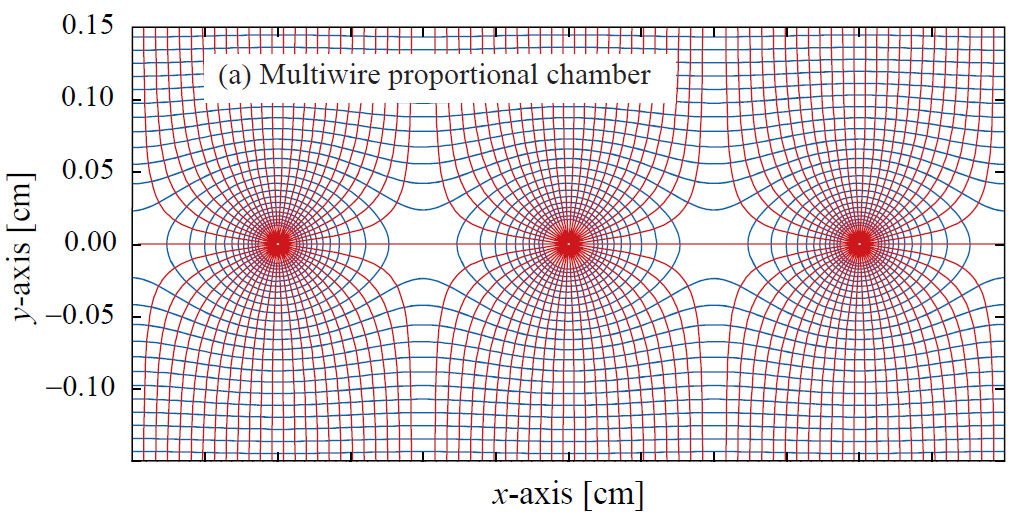
\includegraphics[width=0.8\textwidth]{immagini/campo_elettrico_MWPC.png}
\end{figure}

Notiamo come nella maggior parte della camera il campo elettrico è uniforme, mentre in prossimità del filo diventa molto più intenso, come mostrato dalle linee di campo che diventano più fitte. 

Geometrie tipiche per questi rivelatori consistono in fili da $20 \; \rm \mu m$, distanti 1 mm l'uno dall'altro. La spaziatura, cioè la distanza tra un filo e l'altro, prende il nome di pitch. Questa è una caratteristica generale di tutti i rivelatori segmentati, quindi il pitch rappresenta la distanza tra un elettrodo ed il successivo. \E importante conoscere il pitch di un rivelatore di posizione, perché questo stabilisce la \textit{risoluzione spaziale}\comment{Fino ad ora abbiamo parlato di risoluzione energetica di un rivelatore, cioè la capacità di distinguere due valori in energia vicini tra di loro, poi abbiamo parlato di risoluzione temporale, quindi la capacità da parte di un rivelatore di produrre un segnale che ci dà un'informazione di timing per ad esempio effettuare misure di tempo di volo e adesso abbiamo visto dei rivelatori in grado di costruire la posizione, quindi siamo interessati a un'altra caratteristica, la risoluzione spaziale.}, ossia la capacità di distinguere due posizioni molto vicine tra di loro, dunque la precisione con cui viene ricostruita la coordinata spaziale. Ovviamente essa dipenderà dalla distanza tra un elettrodo ed il successivo, che in questo caso è la distanza tra i fili: più le sequenze di fili sono fitte, migliore sarà la risoluzione spaziale\footnote{Per dare un'idea quantitativa, se due fili fossero distanti tra loro 10 cm, non potremmo dire niente su quello che avviene in questi 10 cm, al massimo riusciremmo ad assegnare la posizione a un filo o all'altro.}. \E da notare che la risoluzione spaziale non è data banalmente dalla distanza $d$ tra un filo e l'altro, bensì è data da
\begin{equation*}
   \sigma_x=\frac{d}{\sqrt{12}}
\end{equation*}
Per cui, se ad esempio i fili sono distanti $d=1 \; \rm mm$, si possono ottenere risoluzioni spaziali dell'ordine di $0,3 \; \rm mm$.

La presenza del fattore $\sqrt{12}$ può essere spiegata in diversi modi. Un modo è il seguente: supponiamo che le posizioni di arrivo delle particelle tra un filo e l'altro seguano una distribuzione uniforme (cioè le particelle, quando arrivano sul rivelatore arrivino con la stessa probabilità in qualsiasi punto della superficie del rivelatore). Una volta definita la funzione di distribuzione di probabilità $D(x)$ (abbreviata in PDF, dall'inglese Probability Distribution Function), data una distribuzione di valori possiamo valutare valore medio e varianza associati alla variabile. Se indichiamo con $x$ la variabile posizione, avremo che tali quantità sono date da
\begin{equation*}
   \expval*{x}
   =\frac{\int_{-\infty}^{+\infty} \dd{x} x D(x)}{\int_{-\infty}^{+\infty} \dd{x} D(x)}
   \qqtext{,}
   \sigma_x^2
   =\frac{\int_{-\infty}^{+\infty} \dd{x} \bigl( x - \expval*{x} \bigr)^2 D(x)}{\int_{-\infty}^{+\infty} \dd{x} D(x)}
\end{equation*}
dove l'integrale a denominatore è dovuto al fatto che in generale la funzione $D(x)$ potrebbe non essere normalizzata a 1. Nel caso in cui lo fosse tale termine si potrà omettere.

Consideriamo adesso un rivelatore segmentato:
\begin{figure}[H]
   \centering
   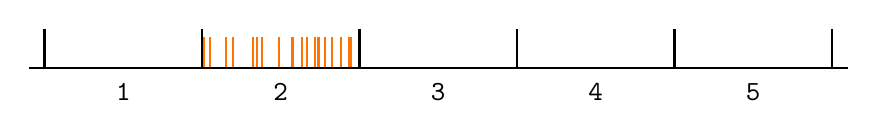
\begin{tikzpicture}
      %eventi
      \foreach \x in {2.1,2.3,2.02,2.7,2.65,2.98,3.15,3.27,3.48,2.76,2.39,3.33,3.56,3.87,3.89,3.43,3.65,3.77} \draw[thick,orange!90!red] (\x,0) -- (\x,0.4);
      %rivelatore
      \foreach \x in {0,2,4,6,8,10} \draw[thick] (\x,0) -- (\x,0.5);
      \draw[thick] (-0.2,0) -- (10.2,0);
      \node at (1,-0.3) {\ttfamily 1};
      \node at (3,-0.3) {\ttfamily 2};
      \node at (5,-0.3) {\ttfamily 3};
      \node at (7,-0.3) {\ttfamily 4};
      \node at (9,-0.3) {\ttfamily 5};
   \end{tikzpicture}
\end{figure}
Consideriamo tutte le particelle che cadono nell'intervallo 2, le quali verranno tutte associate all'omonimo filo. Come abbiamo detto, ci aspettiamo che queste particelle si distribuiscano in maniera uniforme, quindi la loro distribuzione di probabilità deve essere piatta. In virtù di ciò, essa si può esprimere tramite la funzione
\begin{equation*}
   D(x)=
   \begin{dcases}
      \frac{1}{b-a} & \text{per } a \leq x \leq b\\
      0 & \text{per } x>a \vee x>b\\
   \end{dcases}
\end{equation*}
dove $a$ e $b$ sono gli estremi entro cui supponiamo di associare il filo 2 alla particella. Notiamo che tale distribuzione è normalizzata a 1, in quanto si ha
\begin{equation*}
   \int_{-\infty}^{+\infty} \dd{x} D(x)
   =\int_{a}^{b} \dd{x} \frac{1}{b-a}
   =\frac{1}{b-a} \bigl[ x \bigr]_{a}^{b}
   =\frac{b-a}{b-a}
   =1
\end{equation*}
Calcoliamo il valor medio:
\begin{gather*}
   \expval*{x}
   =\int_{-\infty}^{+\infty} \dd{x} x D(x)
   =\int_{a}^{b} \dd{x} \frac{x}{b-a}
   =\frac{1}{b-a} \qty[ \frac{x^2}{2} ]_{a}^{b}
   =\frac{1}{b-a} \frac{b^2 - a^2}{2}=
   \\[0.2cm]
   =\frac{1}{b-a} \frac{(b - a)(b + a)}{2}
   =\frac{b + a}{2}
\end{gather*}
Per quanto riguarda la varianza invece si ha
\begin{gather*}
   \sigma^2
   =\int_{-\infty}^{+\infty} \dd{x} \bigl( x - \expval*{x} \bigr)^2 D(x)
   =\int_{a}^{b} \dd{x} \bigl( x - \expval*{x} \bigr)^2 \frac{1}{b-a}=
   \\
   \qquad
   \underset{\big\uparrow \atop \mathclap{
      \begin{subarray}{c}
         y=x - \expval*{x} \;,\; \dd{y}=\dd{y}\\[0.1cm]
         b \to b - \expval*{x} \;,\; a \to a - \expval*{x}
      \end{subarray}
   }}{=}
   \frac{1}{b-a} \int_{a - \expval*{x}}^{b - \expval*{x}} \dd{y} y^2
   =\frac{1}{b-a} \qty[ \frac{y^3}{3} ]_{a - \expval*{x}}^{b - \expval*{x}}
   =\frac{1}{b-a} \frac{\bigl( b - \expval*{x} \bigr)^3 - \bigl( a - \expval*{x} \bigr)^3}{3}=
   \\
   =\frac{b^3 - 3b^2\expval*{x} + 3b\expval*{x}^2 - \expval*{x}^3 - a^3 + 3a^2\expval*{x} - 3a\expval*{x}^2 + \expval*{x}^3}{3(b-a)}=
   \\
   =\frac{(b^3 - a^3) - 3\expval*{x}(b^2 - a^2) + 3\expval*{x}^2(b-a)}{3}=\\
   =\frac{b^2 + ab + a^2 - 3\expval*{x}(b + a) + 3\expval*{x}^2}{3}
   =\frac{b^2 + ab + a^2 - 3\frac{(b + a)^2}{2} + 3\frac{(b + a)^2}{4}}{3}=
   \\
   =\frac{4b^2 + 4ab + 4a^2 - 6b^2 - 12ab - 6a^2 + 3b^2 + 6ab + 3a^2 }{12}=
   \\
   =\frac{b^2 - 2ab + a^2}{12(b-a)}
   =\frac{(b - a)^2}{12}
   \implies
   \sigma=\frac{b - a}{\sqrt{12}}
\end{gather*}

Un altro modo consiste nel generare un certo numero di numeri casuali in modo uniforme tra due estremi:
\begin{figure}[H]
   \centering
   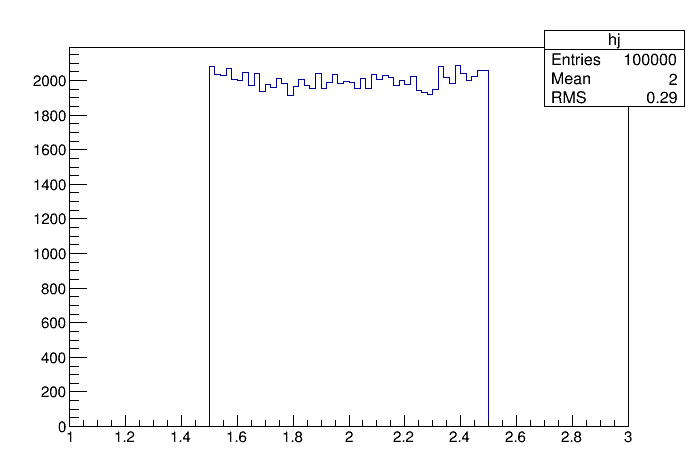
\includegraphics[width=0.69\textwidth]{immagini/numeri_casuali_rivelatore_segmentato.png}
\end{figure}
Nell'esempio in figura sono stati scelti come estremi i valori $a=1.5$ e $b=2.5$ e sono stati generati 100.000 numeri in modo uniforme. Vediamo come la distribuzione di questi valori è abbastanza piatta (non è perfettamente piatta per questioni di fluttuazioni statistiche), il che significa che è equiprobabile che una particella colpisca il rivelatore in corrispondenza di una coordinata piuttosto che in corrispondenza di un'altra.

Il valore medio di questa distribuzione è banalmente dato da
\begin{equation*}
   x
   =\frac{1.5 + 2.5}{2}
   =\frac{4}{2}
   =2
\end{equation*}
come ci aspettavamo, in quanto corrisponde al centro di questa distribuzione. L'rms, cioè la deviazione standard\footnote{Si rimanda all'approfondimento \ref{appr:rms}.}, vale
\begin{equation*}
   \sigma
   =\frac{2.5 - 1.5}{\sqrt{12}}
   =\frac{1}{\sqrt{12}}
   =0.29
\end{equation*}
Tale risultato è una conseguenza del teorema del limite centrale, il quale afferma che la somma (o la media) di un gran numero di variabili casuali, aleatorie, indipendenti tra di loro, segue una distribuzione Gaussiana.

\subsection{Drift Chambers}

Le camere a fili possono essere migliorate. Un esempio sono le Drift Chambers, nelle quali possiamo andare a misurare il tempo di deriva degli elettroni per raggiungere l'anodo a partire dal punto in cui sono stati prodotti. Per fare ciò è necessario avere un riferimento esterno, nel senso che deve esserci una sorta di start che ci permetta di poter misurare quanto tempo è trascorso tra quando gli elettroni sono stati prodotti e quando hanno raggiunto l'anodo. Ecco perché si fa uso di un rivelatore esterno che ci permette di valutare questa differenza di tempo.
\begin{figure}[H]
   \centering
   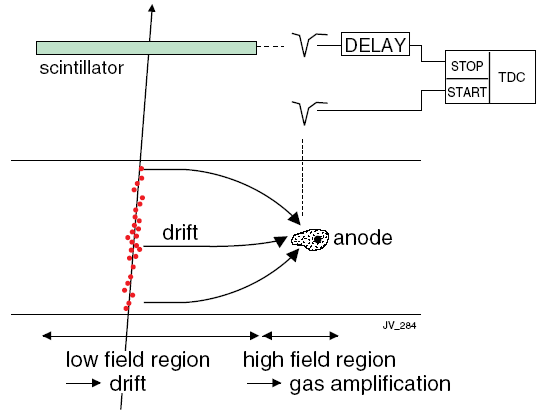
\includegraphics[width=0.65\textwidth]{immagini/drift_chambers.png}
\end{figure}
La situazione è rappresentata schematicamente nella figura sopra: una particella entra nella camera, produce la ionizzazione e quindi gli elettroni, i quali cominciano a migrare per poi arrivare all'anodo, dando luogo a un segnale che funge da start. La particella tuttavia prosegue, incontra un altro rivelatore che produce un segnale e questo rappresenta lo stop. Il modulo indicato in figura con "TDC" (che prende il nome di Time to Digital Converter, come vedremo in dettaglio nel capitolo \ref{chap:modulistica_elettronica}) non fa altro che misurare la differenza di tempo tra il segnale di start e quello di stop. \E chiaro che il segnale di start cambia a seconda di quanto tempo impiegano gli elettroni ad arrivare all'anodo, quindi questo sistema permette di stabilire la distanza dall'anodo, permettendoci di avere una risoluzione spaziale migliore rispetto a quella che abbiamo con le camera fili tradizionali.

Lo svantaggio di tale sistema è che si complica sia il rivelatore, perché dobbiamo avere dei rivelatori esterni di riferimento, sia l'elettronica, in quanto dobbiamo misurare tempi abbastanza piccoli, che è un'operazione non banale.

\subsection{TPC (Time Projection Chambers)}

Altri tipi di rivelatore molto utilizzati sono le TPC, ossia le Time Projection Chambers. Questi sono dei grossi rivelatori i quali hanno dimensioni anche di diversi metri, ad esempio la TPC più grande realizzata al mondo è quella dell'esperimento ALICE, la quale è riportata in figura:
\begin{figure}[H]
   \centering
   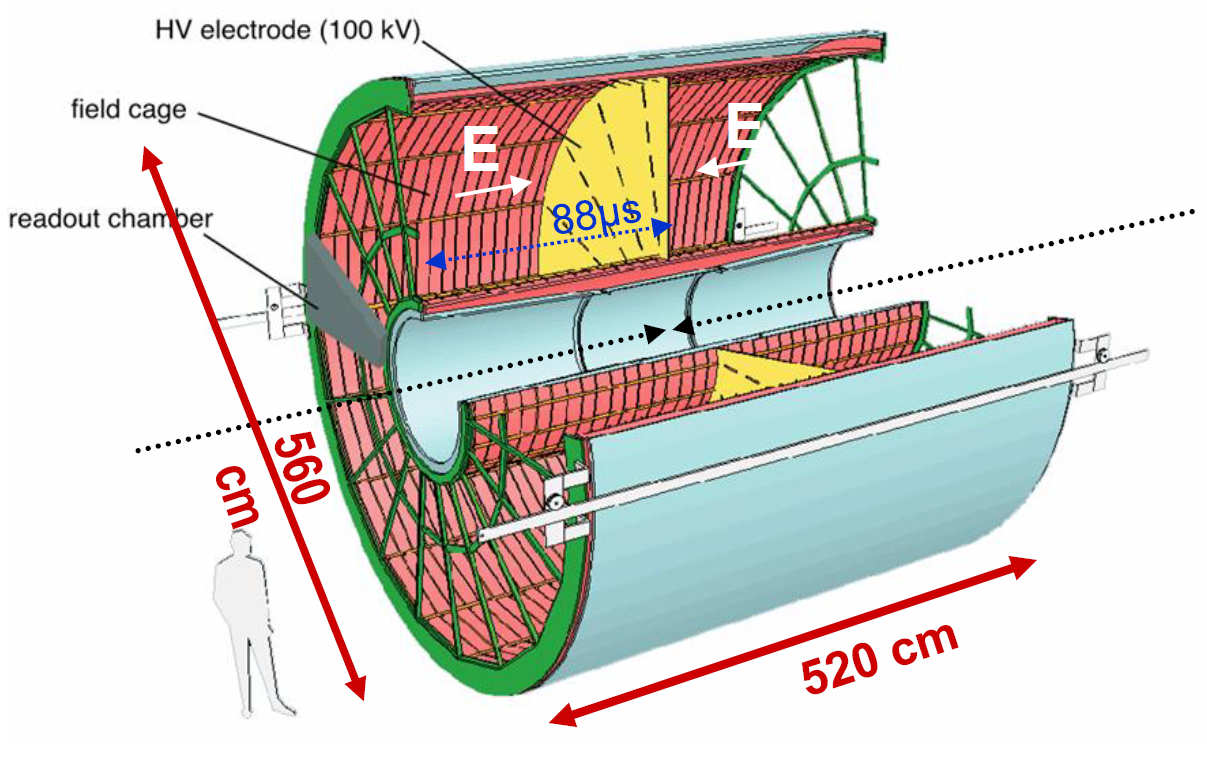
\includegraphics[width=0.6\textwidth]{immagini/TPC_1.png}
\end{figure}
\E da notare che il cilindro interno non necessariamente deve essere presente, in questo caso è presente a causa del fatto che in ALICE all'interno ci sono altri rivelatori, ma in realtà la TPC potrebbe essere un unico volume.

Analizziamo il campo elettrico. Esso ha verso opposto tra un lato e l'altro: il motivo è che in tale rivelatore abbiamo un elettrodo centrale costituito dal piano giallo e poi altri due elettrodi costituiti dalle basi del cilindro, per cui si genera un campo elettrico che è diretto verso l'elettrodo centrale e quindi ha verso opposto nelle due regioni. 

Quando passa una particella, questa ionizza il gas e gli elettroni prodotti cominciano a migrare verso le basi del cilindro, dove sono posizionati dei rivelatori di posizione. Quello che avviene sostanzialmente è che la traccia viene proiettata sul rivelatore di posizione che c'è alla base del cilindro e quindi ricostruiamo tridimensionalmente il passaggio della carica, perché sul piano $xy$ (quello che include la base del cilindro) la posizione viene ricostruita grazie ai rivelatori di posizione, mentre lungo l'asse $z$ (che coincide con l'asse del cilindro) la posizione viene ricostruita andando a misurare il tempo di deriva.
%, cioè quanto tempo impiegano ad arrivare gli elettroni dal punto in cui sono sossa di prodotti fino all'anodo.

Vediamo più nel dettaglio ciò che avviene concentrandoci su metà del rivelatore:
\begin{figure}[H]
   \centering
   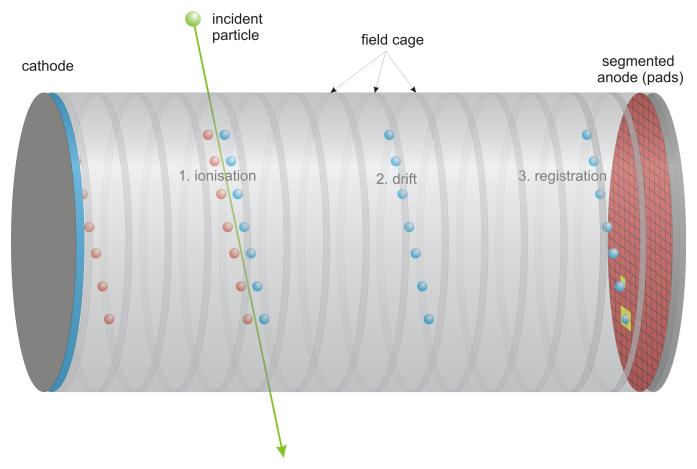
\includegraphics[width=0.6\textwidth]{immagini/TPC_2.png}
\end{figure}
A sinistra abbiamo il catodo (che nella figura precedente era rappresentato dalla superficie gialla) e sull'altra estremità del cilindro abbiamo dei rivelatori segmentati in grado di misurare la posizione. Vediamo come gli ioni si muovano verso il catodo, ma ciò non ci interessa perché sono molto lenti, mentre gli elettroni cominciano a derivare\footnote{Sarebbe l'italianizzazione di "driftare", n.d.r.\,.} a seguito del campo elettrico fino ad arrivare all'anodo, dove vengono rivelati dai rivelatori di posizione, e in base a dove incidono daranno luogo ad un segnale (rappresentato dal quadratino giallo in figura), proiettando così la traccia sulla base del cilindro. La terza dimensione è invece data dal tempo impiegato dagli elettroni per passare dal punto in cui sono stati prodotti all'anodo. In questo modo riusciamo a ricostruire tridimensionalmente la traiettoria della particella.

In generale le TPC forniscono anche una misura della perdita di energia, quindi si misura l'ampiezza del segnale nonché quanti elettroni sono stati raccolti; pertanto sono rivelatori che possono essere utilizzati anche per l'identificazione. Talvolta sono inseriti all'interno di campo magnetico in maniera tale da curvare la particella e misurarne l'impulso, in modo che la $\dv*{E}{x}$ possa essere sfruttata per l'identificazione.

\begin{esempio}[I dati prodotti da una TPC]
   Vediamo quanti dati vengono prodotti da un rivelatore del genere. Prendiamo come riferimento l'esperimento ALICE e supponiamo di avere collisioni tra fasci di piombo, che sono quelle che producono più particelle. Per ogni collisioni vengono prodotte normalmente dalle 10.000 alle 30.000 particelle, quindi abbiamo decine di migliaia di particelle che attraversano la TPC e che devono essere tracciate. Il numero di punti che vengono ricostruiti attraverso questo sistema dipende da quanti anodi sono stati interessati alla base perché, essendo segmentati, dipenderà da quanti segnali sono stati raccolti qui e al massimo se ne possono ricostruire 160. Abbiamo dunque 160 punti sul piano $xy$ per una media di 20.000 tracce per evento, quindi il numero complessivo di coordinate da ricostruire sono
   \begin{equation*}
      \frac{\text{n° coordinate complessive}}{\text{evento}}
      =3 \times 2 \cdot 10^4 \times 160
      =9.6 \cdot 10^6
   \end{equation*}
   Dal momento che gli eventi al secondo sono in numero tra 100 e 1000 possiamo calcolare anche quanti byte di dati si devono trasmettere. Supponendo di assegnare due byte per ogni coordinata si ha
   \begin{equation*}
      \frac{\text{n° bytes}}{\text{secondo}}
      =2 \times 9.6 \cdot 10^6 \times 100
      \approx 2 \; \rm Gb/s
   \end{equation*}
   Tali rivelatori devono quindi avere anche un'elettronica opportuna per gestire questi quantitativi di dati.
\end{esempio}

\subsection{MRPC (Multigap Resistive Plate Chambers)}

Un ultimo esempio è rappresentato dalle Multi Gap Resistive Plate Chambers, cioè le camere a piatti piani resistivi con diverse gap. Queste sono un'evoluzione delle Resistive Plate Chambers (RPC). Vediamo quindi prima in che cosa consistono quest'ultime:
\begin{figure}[H]
   \centering
   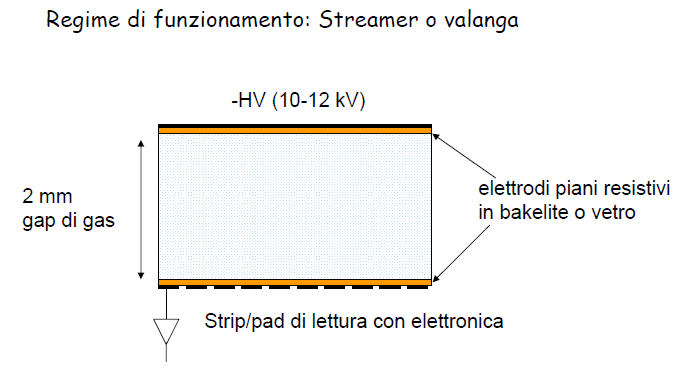
\includegraphics[width=0.7\textwidth]{immagini/RPC.png}
\end{figure}
Anche qui abbiamo una struttura con del gas all'interno e degli elettrodi, ma c'è una particolarità: gli elettrodi non sono metallici, anzi normalmente sono realizzati in un materiale vetroso (bakelite o vetro) e vengono resi altamente resistivi, quindi se ne aumenta la resistività ad esempio attraverso l'utilizzo di vernici. Ciò però fa sì che questi elettrodi, che utilizziamo per creare un campo elettrico molto intenso, non possano essere degli elettrodi di lettura, cioè di raccolta del segnale, perché per essere raccolto il segnale deve essere trasmesso all'interno dell'elettrodo, cosa che non può avvenire se l'elettrodo non è conduttivo. Quello che succede è che gli elettrodi di lettura vengono posizionati all'esterno, come possiamo vedere nella figura in cui sono costituiti da delle strip o da pad\footnote{Le strip e i pad sono rispettivamente delle strisce e dei rettangoli o dei cerchi di materiale conduttivo.}, quindi il segnale che si produce all'interno del gap di gas viene indotto sulle strip esterne o sulle pad esterne.

Sono rivelatori molto piccoli, aventi spessori di qualche millimetro, tuttavia hanno degli svantaggi. Lo svantaggio principale è che il segnale che si raccoglie è dipendente dal punto in cui si è innescata la valanga di cariche, quindi se la valanga si è innescata molto lontano dagli elettrodi essa si sviluppa molto e richiede più tempo per essere raccolta perché più distante, se invece si innesca in prossimità dell'anodo il segnale viene fornito subito. Questo crea un cosiddetto "time jitter", cioè un'indeterminazione nell'informazione temporale associata a quel segnale, perché appunto, a seconda della posizione in cui si è innescata la valanga, il segnale può partire subito oppure con un certo ritardo, e questo è un effetto indesiderato soprattutto per le misure di timing.

Per migliorare questo aspetto si realizzano le Multi-gap Resistive Plate Chambers, in cui la zona sensibile viene suddivisa in tante gap più piccole e ciò si fa con dei "sandwich", una sequenza di vetri che vengono distanziati di poche centinaia di micron. 
\begin{figure}[H]
   \centering
   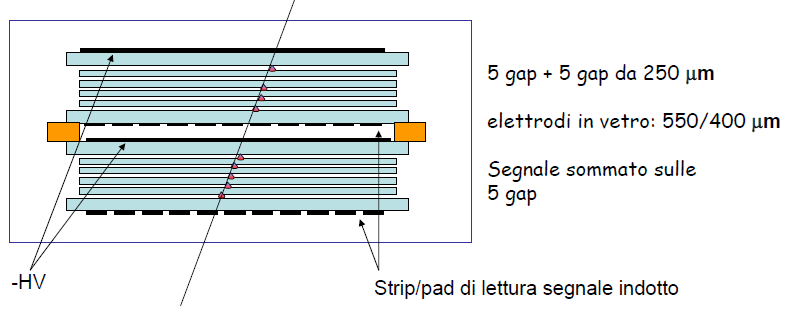
\includegraphics[width=0.85\textwidth]{immagini/MRPC_1.png}
\end{figure}
In questo modo la valanga si sviluppa in una di queste gap. Il segnale complessivo che viene indotto all'esterno è la somma di tutti i segnali che si sono prodotti e quindi l'efficienza rimane elevata (quindi il segnale rimane elevato) però evitiamo il problema del time jitter, il quale non si può presentare per il fatto che le gap sono così piccole.

\comment{
   Questi sono dei rivelatori che possono raggiungere risoluzione delle decine di picosecondi, quindi sono rivelatori molto veloci, infatti vengono utilizzati spesso come rivelatori per misure di tempo di volo. 
   Ad esempio il rivelatore a tempo di volo dell'esperimento Alice ha questa struttura e una multi-gap resisti play chambers, ma anche qui in dipartimento abbiamo un telescopio di camera MRC nell'ambito del progetto extreme energy lens per la misura di raggi cosmici dove ad immaginare una struttura telescopica, quindi tre camera sono abbastanza grandi delle dimensioni di 1,80 m per 1,50 m con uno molto estese, dove l'entro di sono delle strips, lo vedete qui sono evidenziata di sempre una strip con la colpita dalla particella evidenziata in arancione. Queste camere sono state realizzate con dei mezzi abbastanza artigianali, vi faccio vedere alcune fasi di costruzione, vedete qui i diversi vetri che si trovano all'interno della camera che sono ovviamente poggiati uno sull'altro, ma bisogna mantenerli a una distanza di poche centinaia di micron e questo viene realizzato con una trama fatta con un filo da pesca di opportuno diametro che permette di distanziare queste camere su tutta la super, questi vetri su tutta la superficie. Questi sono gli elettro, vi vedete che sono delle strip di rame, ogni volta che passa una particella si induce il segnale sulla strip più vicina e il segnale viaggia a destra e a sinistra e questo permette di ricostruire la posizione perché una coordinate fornita dalla strip che viene colpita, l'altra coordinata quella lunga la strip viene fornita dalla differenza dei tempi di arrivo dei segnali a destra e a sinistra, cioè se la particella colpisce il centro la camera, il segnale arriva lo stesso istante a destra e a sinistra altrimenti appunto dalla misura della differenza di tempo si risale a quest'altra coordinate x e quindi ogni piano ricostruisce mermilla il punto di impatto e questo è un telescopio perché abbiamo tre punti a disposizione possiamo andare a ricostruire la direzione di arrivo della particella in questo caso di Imoni


   quindi il rivelatore Geiger che adopererete è molto portatile, non solo vedano pure da fuori. sì ok quindi una scatoletta ma in realtà il vero e e rivelatore corrisponde a questa zona qui quindi un tubicino della lunghezza di circa 6 centimetri per un diametro di un centimetro veramente piccolo quindi è chiaro che quello che andate a misurare dipenderà dalle dimensioni del rivelatore più piccole il rivelatore meno particelle, parliamo ovviamente di raggi cosmici considerato un determinato fuso è chiaramente più piccolo la superficie e meno particelle andrete a misurare al secondo quindi immediatamente con una geometria di questo tipo si misurano in circa 3 particelle al secondo questo rivelatore funziona, chiaramente il resto della scatoletta è occupato da l'elettronica elettronica che serve per alimentare il contatore Geiger perché ricordo che gli elettri sono rappresentati dal cilindro esterno e dal filo dall'angolo che si trova sul lungo lasse dobbiamo applicare una differenza di potenziare considera, è chiaramente quando non abbiamo da collegare nessun alimentatore all'esterno semplicemente c'è una batteria da 9 volt che va alimentare un piccolo circuito che eleva la tensione quindi la moltiplica di un fattore, non so esattamente all'interno di questo circuito quanto è questo fattore però permette di avere diverse centinaia di volt da applicare a questo tubicino il resto dell'elettronica chiaramente permette invece di andare a prelevare il segnale se vi ricordate è necessaria una resistenza per poter raccogliere solamente la carica legata agli elettroni perché la differenza di potenziale applicata diminuisce leggermente quando arriva il segnale che stia parcoliando e poi tende a tornare al valore di partenza e la velocità di cui si ritorna al valore iniziale dipende dalla costante RC quindi dalla capacità del condensatore rappresentato dal nostro rivelatore e dalla valore del resistore che viene posto in serie quindi all'interno c'è un circuito per andare a prelevare questo segnale ci sarà un formatore per andare a generare un segnale standard perché alla fine del momento che non siamo interessati all'ampiezza del segnale è l'attuale che si produce l'uscita un segnale di tipo logico quindi la cui unica informazione è il il che si formi il segnale quindi ci sia il segnale o non ci sia non ci interessa l'ampiezza, quindi non ci interessa un segnale analogico ma solamente un segnale logico quindi ci sono anche dei connettori in particolare un connettore jet che per poter registrare questo segnale e vederlo all'oscilloscopio se me lo ricordo vi darò a disposizione anche un oscilloscopio per poter guardare questo segnale durante l'esercitazione che farete se non volete collegare questo rivelatore al PC perché questo è uno dei sensori che potrebbe essere collegato a quel sistema che avevamo visto dallo studio che avevamo visto all'inizio se non lo volete collegare al PC ma volete utilizzarlo standalone è possibile accendere il rivelatore e porlo in deposizioni o semplicemente on e allora in questo caso ogni qualvolta che passa una particella si attiva un LED luminoso ogni volta che si accende un LED vuol dire che una particella ha attraversato il contatore Geiger oppure una modalità fastidiosa con il BIP ovviamente non arriva a cadenza di un tempo, sapete, il distribuzione dei tempi di arrivo segue la statistica di Poisson e quindi ogni volta che si attiva il BIP arriva una particella volte ne arrivano due molto ravvicinate, volte passano dei lassi di tempo molto più ampi ma in media se è fatta una misura lunga, in grosso modo la frequenza di conteggio è di 0,3 Hz quindi all'incirca tre particelle ogni 10 secondi capite che facendo delle misure brevi, ad esempio gli 10 secondi, possiamo andare a verificare anche la distribuzione di Poisson anche poi quello che farete durante l'esercitazione quindi, ora così, va bene, ve lo possiamo passare questo ovviamente va alla finestra di ingresso, verso la toglie e poi va alla finestra di di alla fine avrete a disposizione tre contatori Geiger
}